\chapter{Continuous measurements of \Ttwo and \SOtwo}
\label{ch:cont}
The continuous flow loop experiments were designed to address some of the shortcomings of the stopped flow experiments, including the difficulties associated with measuring intermediate levels of oxygenation, and the effects of red blood cells settling when stationary.
As mentioned in the introduction, measurements with continuously flowing blood have been demonstrated by Meyer\cite{MeyerNMRrelaxationrates1995} and the group of Peter van Zijl\cite{ZhaoOxygenationhematocritdependence2007,QinDeterminationwholebrainoxygen2011,GrgacTransversewaterrelaxation2017}.

The first step in this experiment was to confirm that \Ttwo can still be measured in a flowing sample, and to measure the effect of flow on the observed \Ttwo.
This was completed using a sample of water doped with CuSO\textsubscript{4} to give a \Ttwo similar to blood.
The stability of the flow rate in the circuit was also tested.

Following this, experiments with samples of blood were completed to measure \Ttwo at a range of echo times, while \SOtwo was slowly ramped between oxygenated and deoxygenated.
These experiments were completed at fields of \SIlist{5;10;14;20;40}{MHz} (corresponding to approximately \SIlist{0.1;0.2;0.3;0.5;1.0}{T}) to investigate the field dependence of the \Ttwo shortening effect.

\section{Experimental Protocol}

In these continuous flow experiments, the samples of blood used were `fresher' than in the stopped flow experiments, to try and decrease any effects from haemolysis.
The samples were typically used less than 3 days after collection.
To prepare for the experiments, the blood was removed from the fridge and allowed to warm to room temperature while the flow circuit was assembled, and put into the magnet.
In most cases, the magnet was set to the correct magnetic field at least a day before (except for the 20 MHz experiment, which was run immediately after the 40 MHz experiment.)
The water bath controlling the gradient bore temperature was also turned on, this required approximately 40 minutes to warm up and stabilise.
As in the stopped flow experiments, the blood was loaded into the flow circuit, and warmed to the experiment temperature and oxygenated by flowing it through the oxygenator.
During this time, the probe was tuned and matched, and NMR parameters such as pulse power and phase were calibrated.
An initial sample with the iStat was measured, and a \SI{3}{ml} samples was taken for plasma separation in the centrifuge.
Plasma was separated by running the centrifuge at setting `5' for 15 minutes, then removing the plasma layer by pasteur pipette.

The flow rate was set by clamping the tube between the magnet and the lower blood bag.
Initially, the screw clamp was closed and the pgse-profile experiment was started.
The clamp was then loosened until a flow rate around \SI{1}{cm/s} was reached, measured using the phase shift from the NMR experiment.
After this was found, the screw clamp was not adjusted for the rest of the experiment, and the pump rate was set to compensate for the flow and keep a constant volume in both bags.

In these experiments the oxygenation level was slowly ramped down by flowing gas with 0\% \Otwo through the oxygenator while the circuit was flowing.
This flowed into the upper blood bag, where mixing with the oxygenated blood helped to smooth the change in \SOtwo and slow down the process, so that more data points could be collected as the oxygenation decreased.
In the first deoxygenation ramp at each field, samples of blood were taken for blood gas analysis on the iStat to calibrate the optical sensor, as discussed in \autoref{sec:exptsetup-pulseoximeter}.
This was done during deoxygenation, as we found that this had a slower rate than the oxygenation.

To oxygenate the blood, the gas mix through the oxygenator was changed to have 21\% \Otwo.
In later experiments, this was altered slightly to have a stage with 5\% \Otwo, followed by a stage at 21\% \Otwo.
This helped to slow down the oxygenation, and allow more data points to be collected.
Deoxygenation and oxygenation ramps were repeated at least twice for each field/sample.

\subsection{NMR Experiments}
To collect the CPMG and PGSE data, a looping batch script was set up in Prospa to automatically run the experiments.

Multiple versions of the standard CPMG experiment included in Prospa were added with echo times equal to \SIlist{1;5;8;10;20}{ms}, and the number of echoes varied to give a total echo train length of \SI{600}{ms}.
4 scans of each CPMG experiment were used with the standard phase cycling and a \SI{1.2}{s} inter-experiment delay (the sample was flowing through the coil, bringing in `fresh' spins, so the repetition time could be less than $5 \times \mathit{T_1}$.)
Additionally, a PGSE experiment was added to monitor the flow rate, with $\Delta = \SI{16}{ms}$, $\delta = \SI{2}{ms}$, $\mathit{g} =$ \SIrange{0}{0.015}{T/m} over 4 steps, and a \SI{15.5}{ms} echo time.
The x gradients were used as the PGSE gradient, as this corresponds to the direction of flow through the coil.
\autoref{eq:PGSEvel} (restated here) was used to calculate the flow velocity.
\begin{displaymath}
v = \frac{\phi}{\gamma \Delta \delta g}
\end{displaymath}
These parameters allow for measurement of velocities \SI{< 5}{cm/s} without phase wrapping.
A standard 1pulse FID experiment is also run, to test for any shifts in the magnetic field.

The batch script in Prospa runs each experiment, then moves to a new directory and repeats.
Each cycle of 7 experiments takes approximately 45 seconds, to complete.
Data is also continuously collected from the optical \SOtwo sensor, and the Picolog temperature logger.

The data is processed using Python in JuPyter notebooks.
Each echo train is phased, and each echo is summed to give a single value for the signal at each echo time.
Similarly to the stopped flow experiments, signal before \SI{15}{ms} was trimmed to remove the signal from the tube.
To try and minimise the effect of flow, the section of the decay used to find \Ttwo was also limited to the first \SI{360}{ms} of the echo train.
The \Ttwo and fitting uncertainty was then found by non-linear exponential fitting of the echo train.
Additionally, the time of each CPMG experiment was extracted from the file system, so that it could be compared with the \SOtwo measurements.


\section{Flow testing}
\subsection{\Ttwo and flow}
\label{sec:contflow-Ttwoflow}
Having the sample flow through the coil causes a decrease in the measured \Ttwo, due to the effect of added dispersion, and the outflow of excited spins from the coil.
In particular, the outflow effect becomes signifcant as the time in the coil (\SI{2}{cm} long) becomes shorter than the experiment time, as the decrease in spins from the coil adds to the true \Ttwo decay and causes the \Ttwo to appear shorter.
To test the impact of flow on the \Ttwo measurements in this experiment, a 1\% NaCl solution doped with \SI{5}{mmolL^{-1}} CuSO\textsubscript{4}, was prepared to test with.
This was loaded into a circuit without the oxygenator and CPMG and PGSE experiments were measured at a range of flow rates.

\begin{figure}[ht]
%Graph from processBloodOxygenation2/171116 Doped water twobag s1.ipynb
\centering
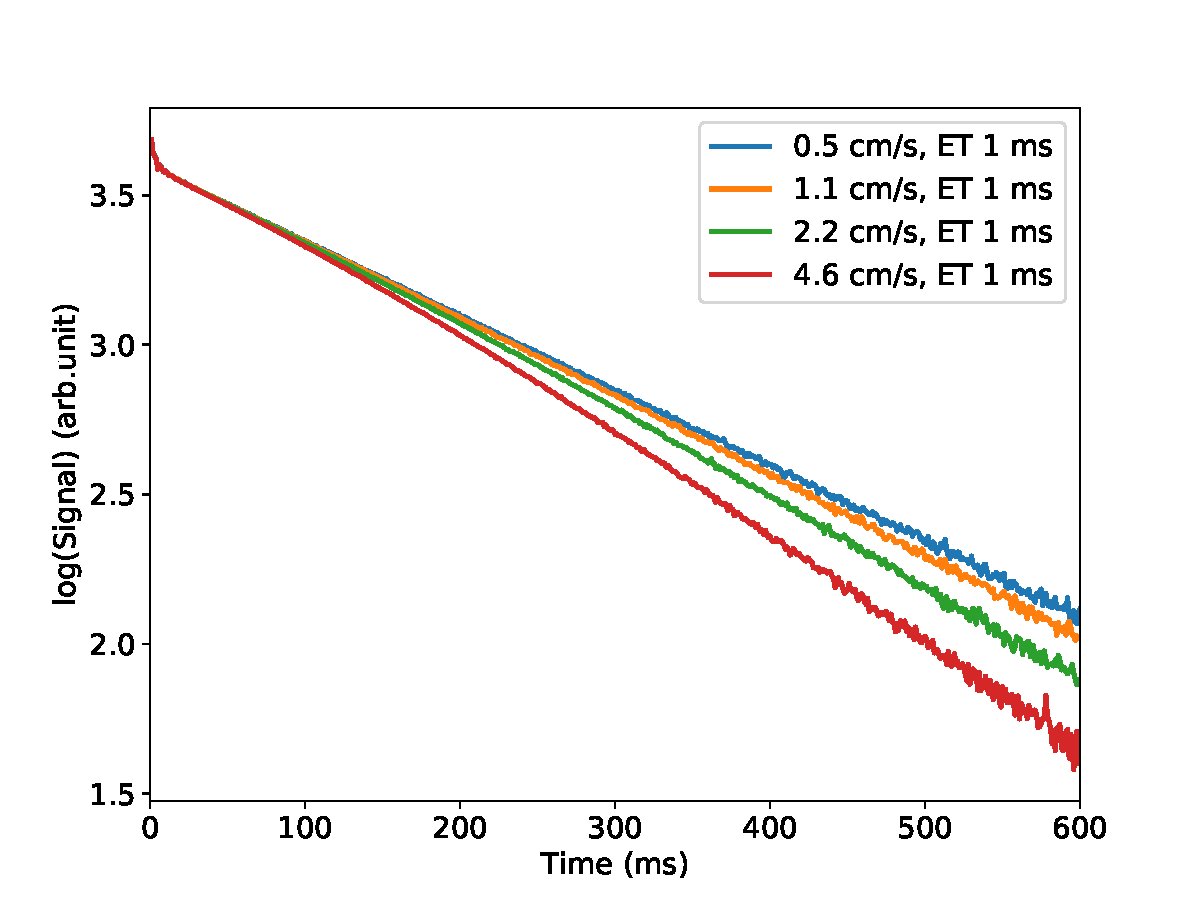
\includegraphics[width=0.8\textwidth]{figures/contflow/dopedwatercpmgdecay.pdf}
\caption{Examples of CPMG echo trains for doped water samples at different flow rates}
\label{fig:contflow-watercpmgdecay}
\end{figure}

\autoref{fig:contflow-watercpmgdecay} shows CPMG echo trains measured for the doped water measured at 4 flow rates, shown on a log scale.
In the first \SI{100}{ms}, all four decays appear the same, but as the flow rate increases, the lines become curved as the signal stops being monoexponential.
As expected, this effect is much larger at the highest flow rate (\SI{4.6}{cm/s}.)
Interestingly, this speed corresponds with a time in the coil of only \SI{430}{ms}, but signal is still being detected after this, suggesting that there is a distribution of speeds in the sample. TODO is this that propagator thing??
There appears to be little effect at the two lower flow rates, and at \SI{2.2}{cm/s}, the effect is not significant until approximately \SI{300}{ms} into the decay.
These decays were fitted with non-linear fitting to obtain \Ttwo values at different flow rates, shown in \autoref{fig:contflow-Ttwovelocity}.

\begin{figure}[t]
%Graph from processBloodOxygenation2/171116 Doped water twobag s1.ipynb
\centering
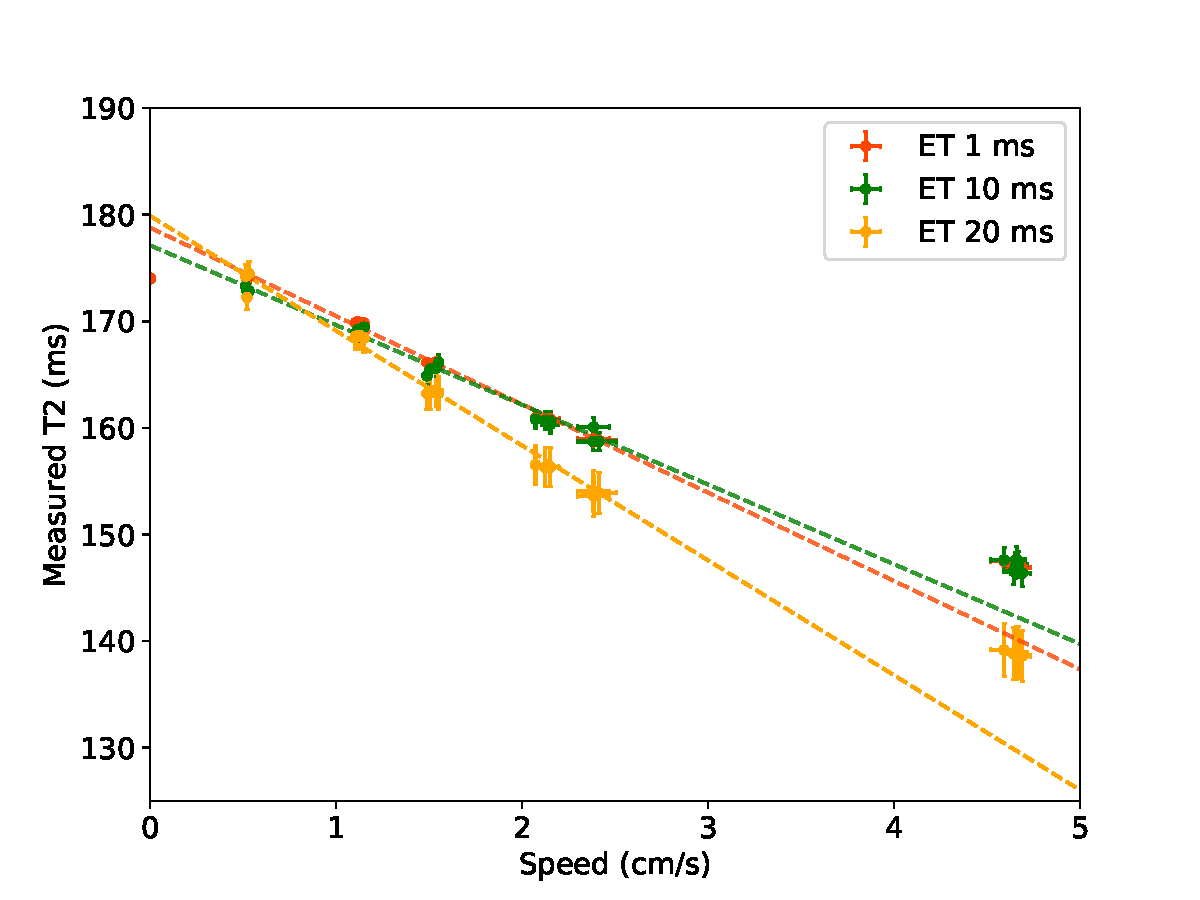
\includegraphics[width=0.8\textwidth]{figures/contflow/T2velocity.pdf}
\caption[Measured \Ttwo values at different flow rates]{Measured \Ttwo values at different flow rates. v=0 point measured in separate experiment. Lines fitted to points where v\SI{<3}{cm/s}.}
\label{fig:contflow-Ttwovelocity}
\end{figure}

As expected, the \Ttwo values measured at higher flow rates decrease from \SI{174}{ms} to around \SI{150}{ms}, with a stronger effect measured at the \SI{20}{ms} echo time.
The decrease appears roughly linear for all but the fastest speed, and these data points were fitted to determine the trend, and the intercept where v=0.
These fit parameters are included in \autoref{tab:contflow-Ttwovelocitylinfit}.

Because the \Ttwo decrease due to flow becomes negligible at low speeds (as the time in coil increases proportional to $\frac{1}{\mathit{v}}$), the intercepts of the lines of best fit overestimate the true \Ttwo (\SI{174}{ms}, measured in a separate experiment) by \SI{4}{ms}.
Additionally, the slopes would be dependent on the true \Ttwo of the sample, as a sample with a short \Ttwo would be less affected by the effect of flow, and vice versa.
As the \Ttwo of the blood will be changing during the experiment, applying the linear correction shown here would not necessarily work.
However, from these experiments, the change in \Ttwo due to flow should be less than \SI{10}{ms}, for flow rates less than \SI{1.5}{cm/s}.
In blood \Ttwo changes due to blood oxygenation are larger than this effect -- on the order of \SI{50}{ms} at 10 MHz -- and the flow rate should stay relatively constant over the course of the experiment, so effects from flow should be relatively small.

\begin{table}[h]
\centering
\caption{Measured \Ttwo dependence on speed}
\label{tab:contflow-Ttwovelocitylinfit}
\begin{tabular}{|c|cc|}
\hline
Echotime (\si{ms}) & Intercept (\si{ms}) & Slope (\si{ms/cm/s}) \\
\hline
1        & 178 \pm 1    & -8.2 \pm 0.2    \\
10       & 177 \pm 1    & -7.4 \pm 0.3    \\
20       & 179 \pm 1    & -10.7 \pm 0.3  \\
\hline
\end{tabular}
\end{table}

\subsection{Flow stability}
\label{sec:contflow-flowstability}
The stability of the flow produced in the circuit was also tested, after early experiments showed a series of spikes in the \Ttwo data.

An example is shown in \autoref{fig:contflow-spikeyTtwo}, from an experiment with blood at 14 MHz.
There are large spikes of up to \SI{40}{ms} in the measured \Ttwo{}s, which makes it difficult to see trends due to changing \SOtwo.
Interestingly, there is a period of `calm' between 355 and 380 minutes, before it goes back to the random spike pattern.

\begin{figure}[ht]
%Graph generated in processBloodoxygenation2/171110 14mhz
\centering
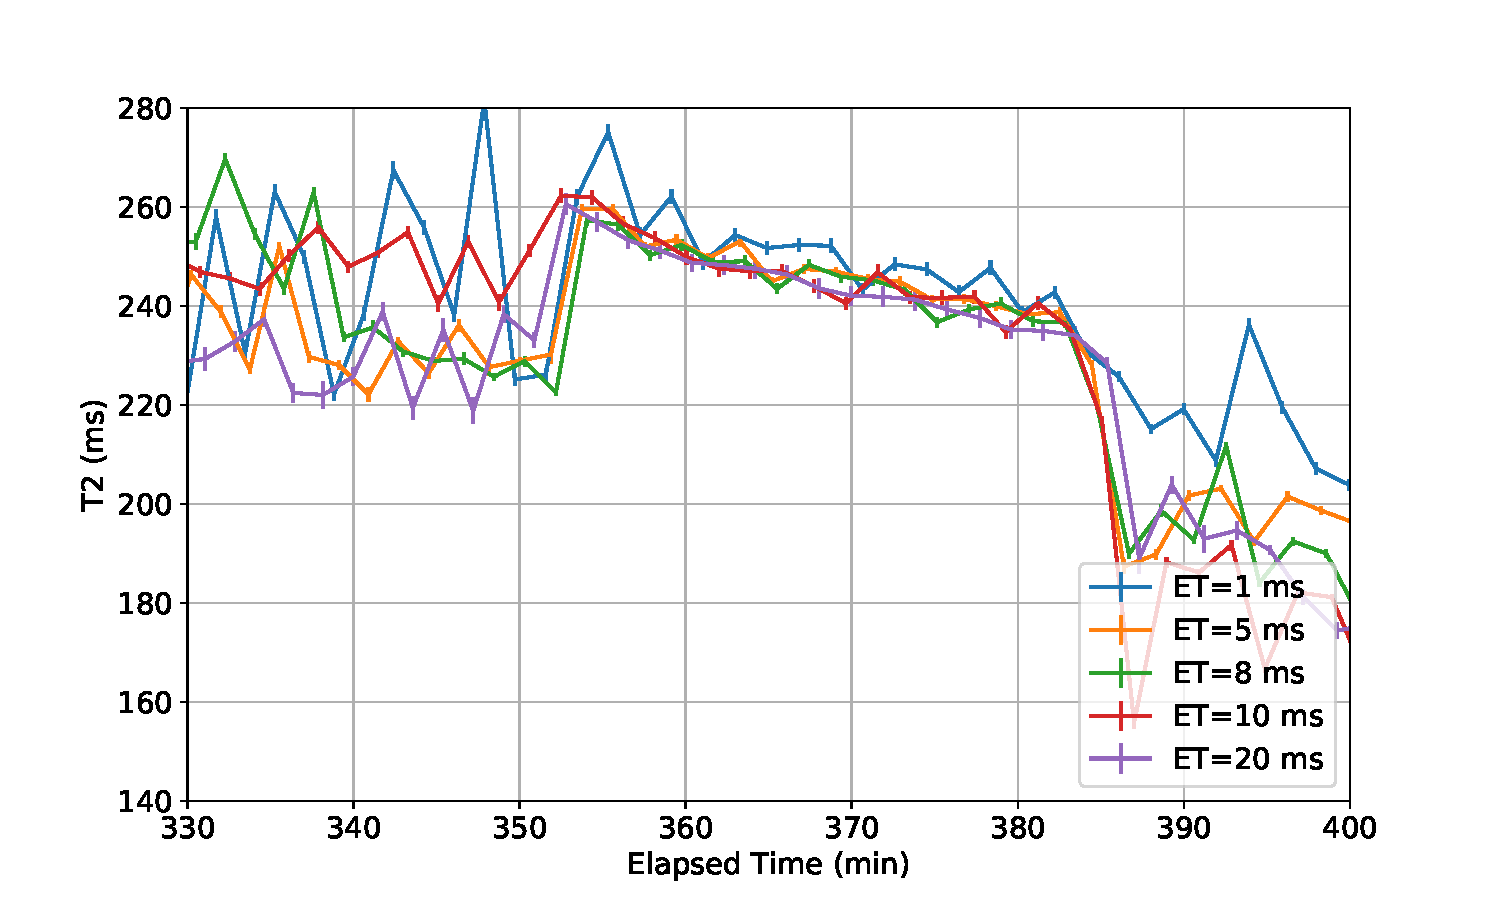
\includegraphics[width=\textwidth]{figures/contflow/spikeyTtwo.pdf}
\caption[Spikes in continuous \Ttwo measurements]{Spikes in continuous \Ttwo measurements from unstable flow}
\label{fig:contflow-spikeyTtwo}
\end{figure}

There were a number of possible causes for this effect, including absolute phase effects from the timing in the Kea spectrometer, and changing sauces of RF  noise.
This was eventually tracked down to an issue with the stability of the flow in the circuit.
In these experiments, the lower bag was not included in the circuit, so that the magnet output was connected directly to the peristaltic pump.
To see how this affected the flow circuit, PGSE experiments were used to measure the velocity of doped water sample flowing in the circuit.

\begin{figure}[ht]
%plots made in flowtesting round 2/fast pgseprofile pump
\centering
\begin{subfigure}[t]{0.32\textwidth}
\caption{No flow}
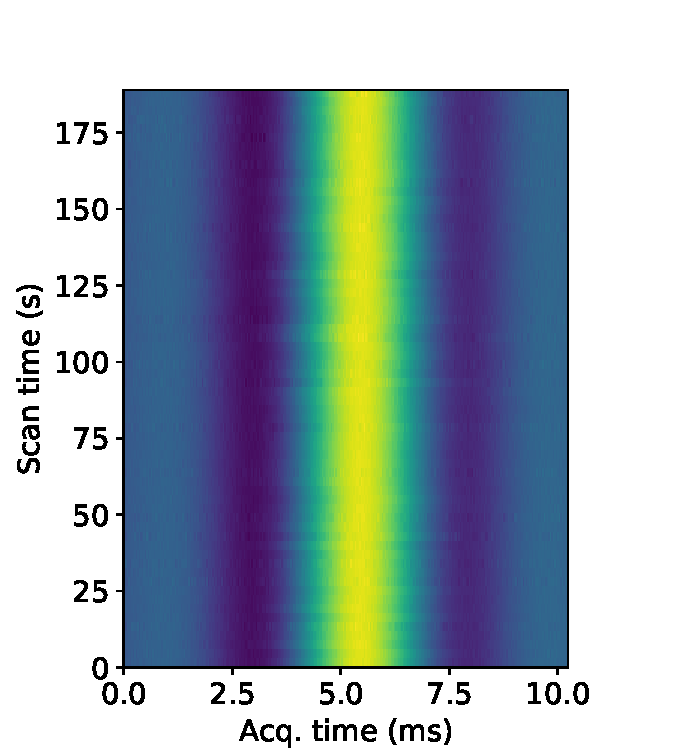
\includegraphics[width=\textwidth]{figures/contflow/flowstabilitynoflow.pdf}
\end{subfigure}
\begin{subfigure}[t]{0.32\textwidth}
\caption{Pump flow}
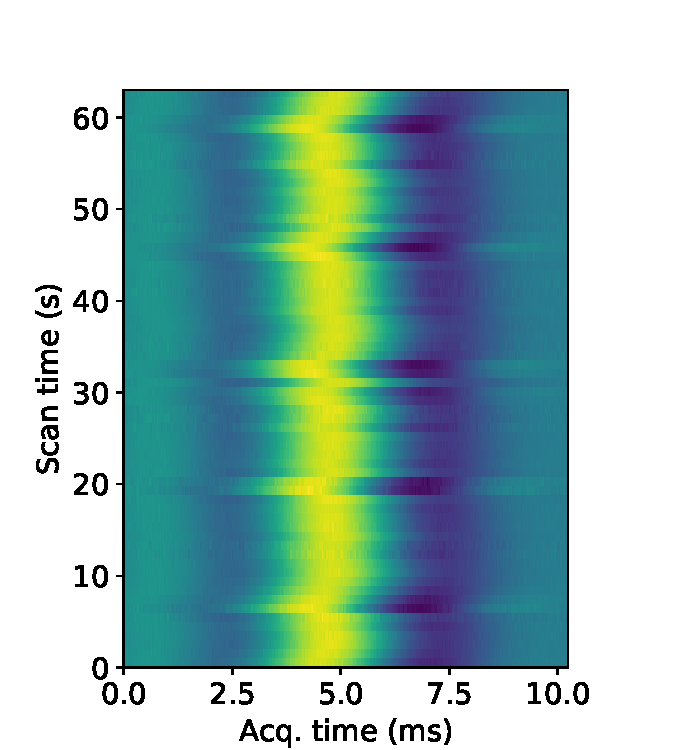
\includegraphics[width=\textwidth]{figures/contflow/flowstabilitybadpump.pdf}
\end{subfigure}
\begin{subfigure}[t]{0.32\textwidth}
\caption{Gravity flow}
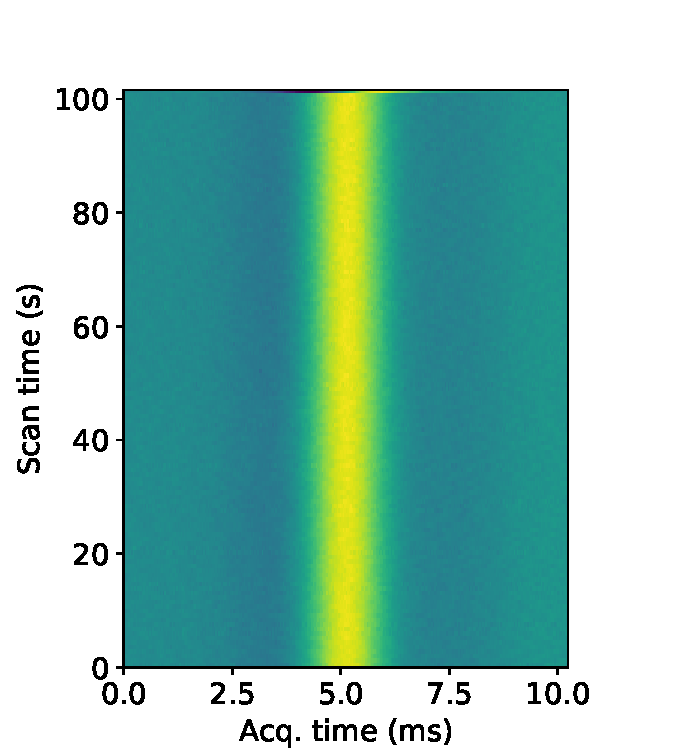
\includegraphics[width=\textwidth]{figures/contflow/flowstabilitynewsetup.pdf}
\end{subfigure}

\caption[PGSE data showing flow stability]{PGSE data showing stability for different flow setups. Collected with PGSE experiments using a repeated \textit{g/q} step so phase changes show velocity. The x-axis shows the acquisition time, while the experiment time is on y. Colour shows the intensity of the real part of the signal.}
\label{fig:contflow-flowstabilityrawpgse}
\end{figure}

\autoref{fig:contflow-flowstabilityrawpgse} shows the raw spin echoes collected in these experiments.
In this experiment, a constant value of \textit{g}=\SI{0.01}{T/m} was used so that changes in phase reflect changes in the velocity.
The experiment with no flow shows no changes in phase, as expected.
However, when the pump is turned on, there are clearly disturbances, which occur with a period of 13 seconds.
Processing this to find the velocities gives \autoref{fig:contflow-flowstabilityspeed}, which shows that the flow rate from the pump drops by over 50\% every 13 seconds.
This is half of the rotational period of the pump head (approximately 26 seconds when set to 2.3 rpm), which is expected as it has two rollers.
This drop is from a short period of time where both rollers stop squeezing the tube as the head rotates.
When this is combined with the effect of phase cycling, this could cause the spikes in the measured \Ttwo.

The flow circuit was modified to include another blood bag between the magnet and the pump, and the have the blood flow under gravity.
This give a much more stable flow, as can be seen in \autoref{fig:contflow-flowstabilityrawpgse}(c), and the green curve in \autoref{fig:contflow-flowstabilityspeed}, which has a speed of \textit{v} = \SI{1.04\pm0.02}{cm/s} over the 100 seconds it was measured for.

\begin{figure}[ht]
%plots made in flowtesting round 2/fast pgseprofile pump
\centering
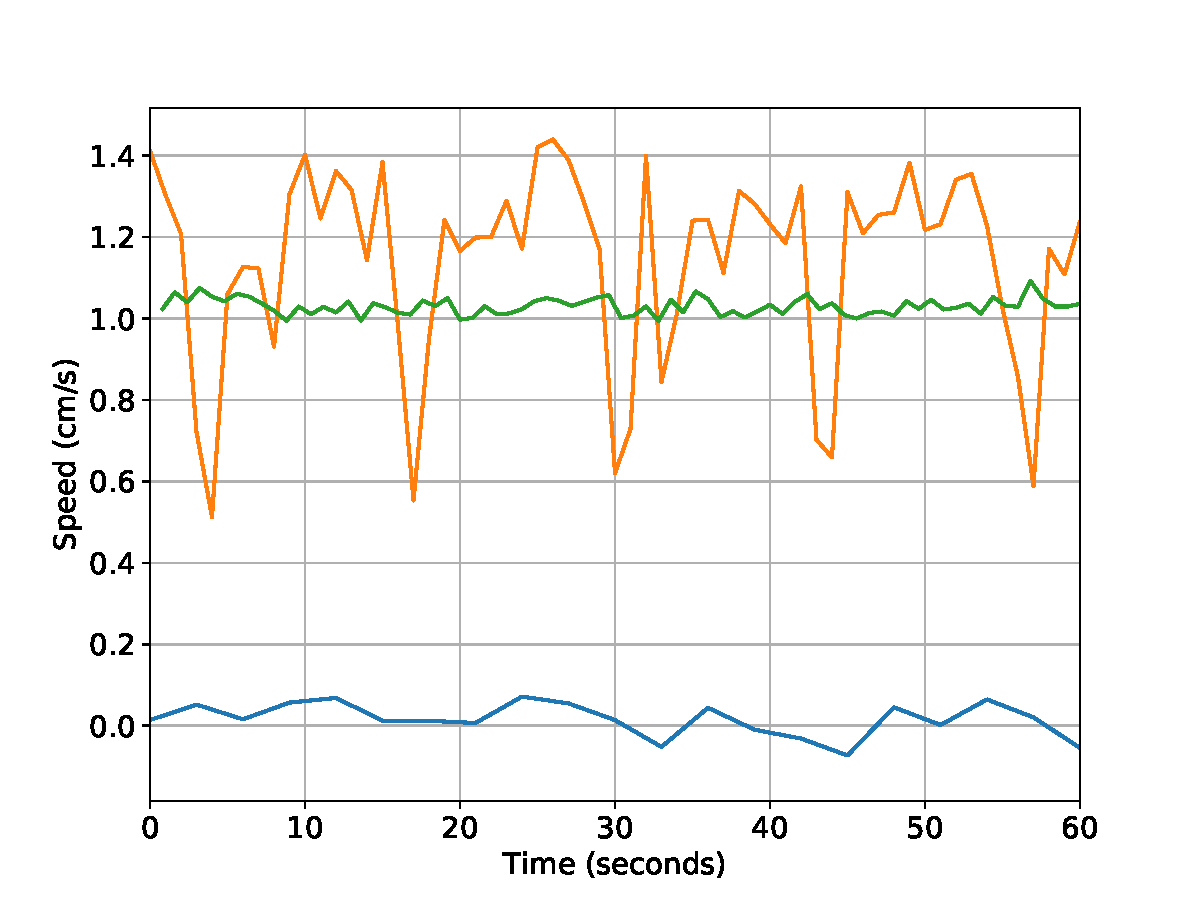
\includegraphics[width=\textwidth]{figures/contflow/flowstabilityspeed.pdf}
\caption[Flow rate stability for different continuous flow setups]{Flow rates measured by PGSE for: No flow (blue), Pump flow (yellow), Gravity flow (green)}
\label{fig:contflow-flowstabilityspeed}
\end{figure}

\section{Blood results}

One sample of blood was used to do measurements at each field strength.
These results are shown as plots of \Ttwo against the experiment time, which was started when the blood sample was loaded into the circuit.
The calibrated \SOtwo measurements from the optical sensor as also shown on the same plots.
No correction is made to this data to adjust for the distance/delay between the oxygen sensor and the NMR probe, which was typically 1-1.2 minutes.
Additionally, the flow rate was monitored during the experiments but was not used to adjust the \Ttwo values.
Temperature was also measured during each experiment, and generally stayed within \SI{29\pm4}{\celsius} (temperature control was better in some experiments, this is shown in the captions).

\subsection{40 MHz}
\begin{figure}[t]
\centering
\makebox[\textwidth][c]{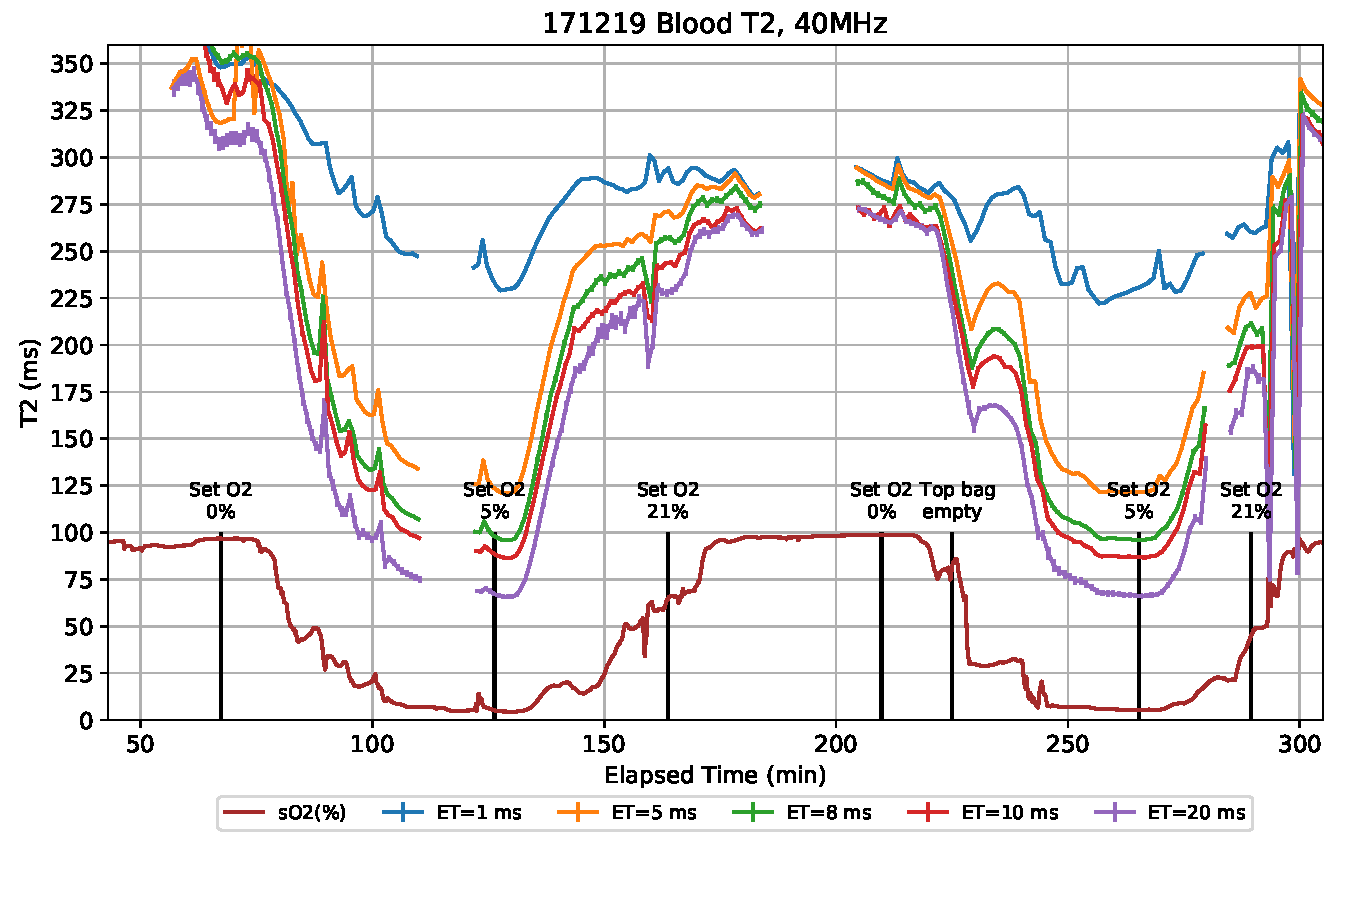
\includegraphics[width=1.2\textwidth]{figures/contflow/40MHzT2Time.pdf}}
\caption[\Ttwo measurements during blood oxygenation ramping at 40 MHz field]{\Ttwo measurements during blood oxygenation ramping at 40 MHz field. Error bars show \Ttwo fitting error. HcT = 0.35. v=\SI{1.0\pm0.15}{cm/s} between  55-280 minutes. Temperature increased from \SIrange{26}{29}{\celsius} from 55-280 minutes.}
\label{fig:contflow-40mhzT2Time}
\end{figure}

The blood used in the 40 MHz and 20 MHz experiments was collected the day before the experiment.
The results are shown in \autoref{fig:contflow-40mhzT2Time}.

At a field of 40 MHz (approximately \SI{1}{T}), there is a clear drop in \Ttwo from when the oxygen saturation is lowered.
The inital \Ttwo is around \SI{350}{ms}, which is quite high compared to the stopped flow results (Spinsolve at 42 MHz measured \SI{310}{ms} for initial \Ttwo.
There is also a \SI{40}{ms} splitting between the short and long echo times, which should be much smaller at this oxygenation.
This could be due

As the \SOtwo is lowered, around 90 minutes, there are spikes visible in both the \Ttwo and \SOtwo.
These are due to samples of blood being syringed out of the circuit to calibrate the optical sensor.
The splitting between the short and long echo times also increases as the blood is deoxygenated.

The blood was assumed to be deoxygenated at 120 minutes.
Here, the splitting between the echo times becomes much clearer -- the \SI{1}{ms} echo time has a \Ttwo of \SI{250}{ms}, while the \SI{20}{ms} echo time is at \SI{75}{ms}.
This agrees with the trends seen in the stopped flow results, although the actual \Ttwo values is higher in this experiment.
The gap from minute 110-121 (and also 184-205) was due to stopping the looping batch file and running the experiments discussed in \autoref{ch:models}.

The \SOtwo was then increased again, with a stage at 5\% \Otwo followed by a stage at 21\%.
The \Ttwo increases to around \SI{280}{ms} when reoxygenated (at 181 minutes), rather than the initial \SI{350}{ms} value.
This effect was also seen in the stopped flow experiments.

During the second deoxygenation ramp, the top blood bag ran empty due to the pump being set too slow (minute 225).
This stopped the smooth deoxygenation ramp, and meant that the relatively deoxygenated blood from the oxygenator was sent through the circuit withough mixing with oxygenated blood in the bag.
This can be seen in the optical data, as there is a sudden drop to around 30\% saturated, and it then stays constant.
The \Ttwo responds differently however, with a slight increase, followed by the expected decrease.
This may be due to the deoxygenated blood mixing with the oxygenated blood in the tube as it travels from the optical sensor to the magnet.
The \Ttwo values measured at the second deoxygenated stage (260 minutes) agree well with values in the first deoxygenated stage, although there is a spike in the \SI{1}{ms} echo time data which does not appear in the others.

The blood was then reoxygenated in two stages.
The NMR experiment was switched off around minute 280, and there appear to be artifacts at minute 293 and 300.
At the third oxygenated stage, the \Ttwo reached \SI{320}{ms}, which is still lower than the initial value, but is higher than the second oxygenated level.

Because of the artifacts in ramp up 1, ramp down 2 and ramp up 2, only the first deoxygenation ramp has been used for further analysis.

\subsection{20 MHz}
\begin{figure}[t]
\centering
\makebox[\textwidth][c]{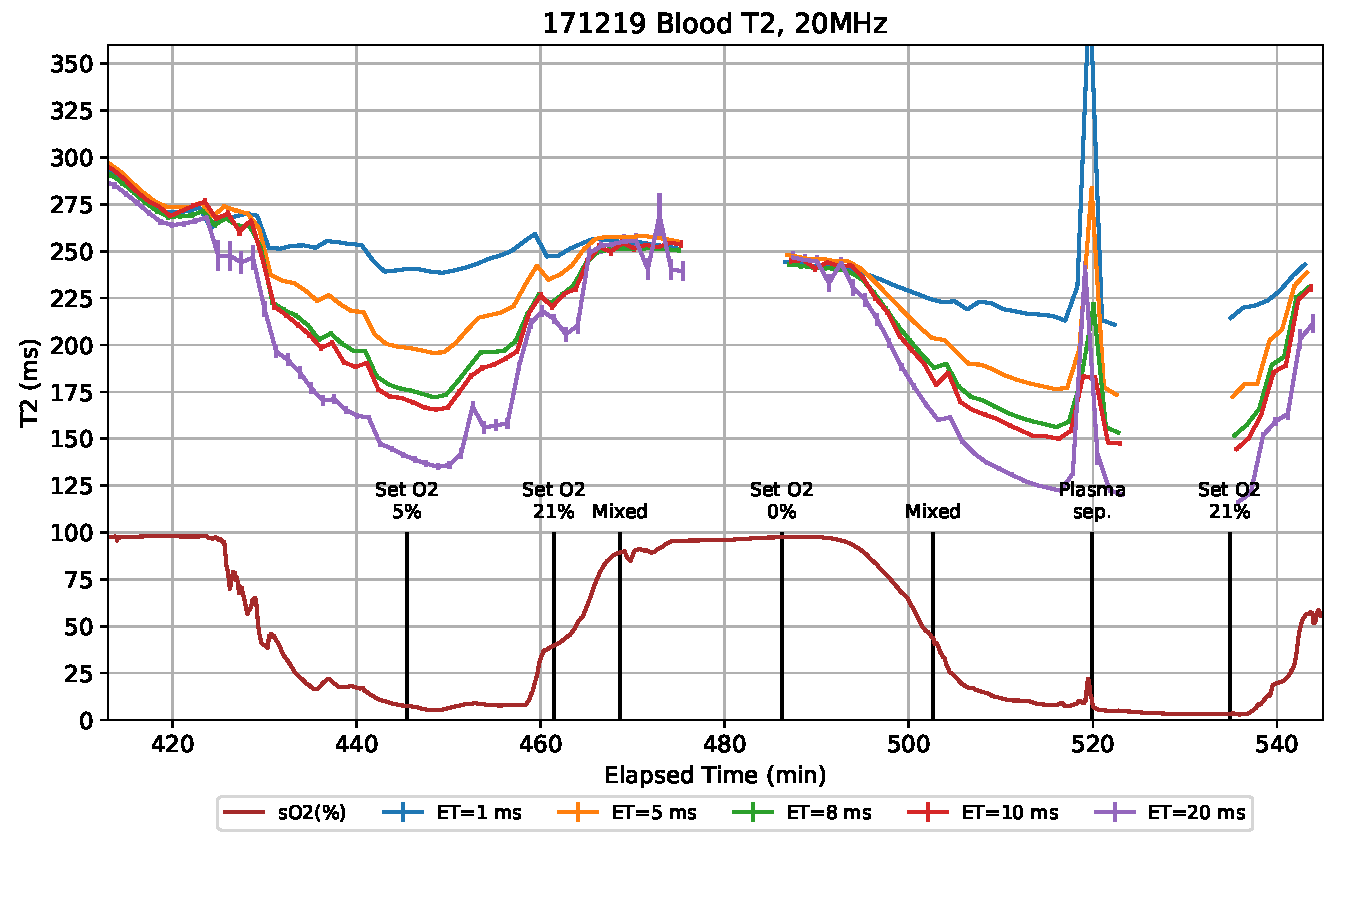
\includegraphics[width=1.2\textwidth]{figures/contflow/20MHzT2Time.pdf}}
\caption[\Ttwo measurements during blood oxygenation ramping at 20 MHz field]{\Ttwo measurements during blood oxygenation ramping at 20 MHz field. Error bars show \Ttwo fitting error. Hct = 0.35. v=\SI{1.9\pm0.1}{cm/s} between  415-515 minutes. Temperature decreased from \SIrange{33}{29}{\celsius} from 415-515 minutes.}
\label{fig:contflow-20mhzT2Time}
\end{figure}

Immediately after the experiment at a field of 40 MHz, the current in the magnet was dropped to produce a 20 MHz field.
The probe was re-tuned and matched for the lower frequency, and pulse power calibration was checked (although the same coil was used, there may have been changes in the tuning and matching at a different frequency).
The results are shown in \autoref{fig:contflow-20mhzT2Time}.

In the 20 MHz experiment, the initial \Ttwo is around \SI{275}{ms} for all echo times, which is lower than in the 40 MHz experiment.
While this is likely caused by the same process lowering \Ttwo in the 40 MHz experiment, there may also be a contribution from the increased flow rate in this experiment.
There is still a significant drop as the blood is deoxygenated, and the splitting betweeen different echo times is still clear.
For the deoxygenated blood, the \Ttwo at the \SI{1}{ms} echo time is \SI{237}{ms}, while the \SI{20}{ms} echo time gives a \Ttwo of \SI{135}{ms}.
As expected, the size of the change from oxygenated to deoxygenated is smaller than in the 40 MHz experiment.

When the blood is reoxygenated, the \Ttwo increases to \SI{250}{ms} for all echo times.
As in the 40 MHz experiment, the looping batch experiments was interrupted between minutes 475-485 and 522-534 to do CPMGvT experiments.

The same pattern is seen in the second deoxygenation-oxygenation ramp.
At minute 520, there is a large spike in \Ttwo, this is due to plasma and red blood cells separating in the blood.
When the blood is no longer homogeneous, the plasma creates a second relaxation component with a much longer \Ttwo (\SI{>500}{ms} for separated plasma) that increases the measured \Ttwo.
This was fixed by squeezing the tubes slightly to mix the blood.
There were also issues caused by the blood in the blood bags separating into regions with different oxygenation.
When these were pulled into the outlet of the bag, they created slugs of blood in the tube with a different oxygenation.
To try and avoid this, the bags were mixed by gentle shaking.

TODO what are the good bits of this graph?

\subsection{14 MHz}
\begin{figure}[ht]
\centering
\makebox[\textwidth][c]{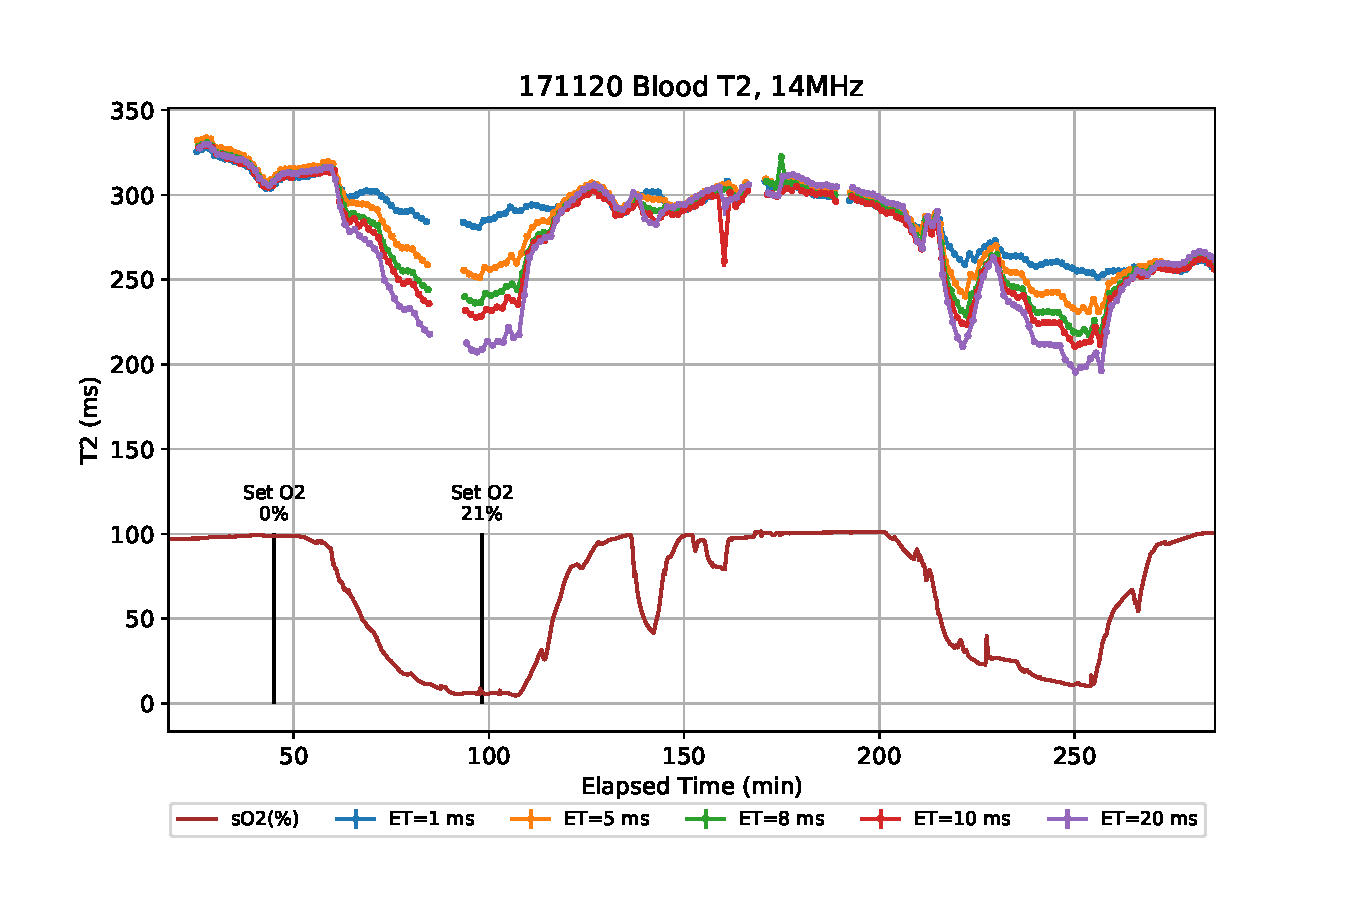
\includegraphics[width=1.2\textwidth]{figures/contflow/14MHzT2Time.pdf}}
\caption[\Ttwo measurements during blood oxygenation ramping at 14 MHz field]{\Ttwo measurements during blood oxygenation ramping at 14 MHz field. Error bars show \Ttwo fitting error. Hct =TODO - check iStat. v=\SIrange{1.2}{0.7}{cm/s} between  20-286 minutes. Temperature varied from \SIrange{25}{29}{\celsius} during experiment. Last two gas mix change times not recorded.}
\label{fig:contflow-14mhzT2Time}
\end{figure}

The blood sample was collected 11 days before the experiment, and the results are shown in \autoref{fig:contflow-14mhzT2Time}.
In the 14 MHz field experiment, the initial \Ttwo is approximately \SI{315}{ms} for all echo times.
As the \SOtwo is decreased, \Ttwo decreases, and the splitting between echo times becomes visible.
When the blood is deoxygenated, the \Ttwo at the \SI{1}{ms} echo time is \SI{283}{ms}, and \SI{206}{ms} for the \SI{20}{ms} echo time.
Both the size of the decrease from  oxygenated to deoxygenated, and the \SI{80}{ms} splitting between the echo times is smaller than found in the 20 MHz experiments, as expected from theory.
When compared with the stopped flow experiments at a field 12 MHz the difference between oxygenated and deoxygenated is roughly the same, which suggests that the flow is not having a large effect.

Reoxygenating occured using only one step with 21\% \Otwo.
This caused a relatively fast increase in the \SOtwo, particularly at low \SOtwo values where the \Ttwo change is most rapid.
This limited the number of points that could be collected during this part oxygenation ramp, e.g. around minute 110.

There is only a slight drop in the \Ttwo at the second oxygenated stage when compared to the initial value (\SI{315}{ms} to \SI{300}{ms}).
However, the second deoxygenated stage has a slightly smaller splitting between the echo times, although this may be because the first deoxygenation stage reached a lower \SOtwo.

At minute 141, the optical sensor shows a slug TODO better word? of unmixed deoxygenated blood from the upper blood bag going past.
This is also shown in the NMR data, which shows the \Ttwo from short and long echo times split by \SI{20}{ms}.
The splitting here is smaller when compared to the splitting at the same \SOtwo from the first deoxygenation section, which is \SI{50}{ms}.
This suggests that the saturation has increased by the time it has reached the NMR probe.

A similar effect can be seen at minute 218, where the splitting between short and long echo times drops to under \SI{5}{ms}.
This suggests a slug of oxygenated blood has gone through the probe.
Interestingly this is not really shown on the optical sensor, which only shows a small spike.

Because of the rapid increases in \Ttwo during the oxygenation ramps, and the \Ttwo spike in the second deoxygenation ramp, only the data from the first deoxygenation ramp is used for further analysis.


\subsection{10 MHz}

\begin{figure}[ht]
%Generated in processbloodoxygenation2/171122 10mhz
\centering
\makebox[\textwidth][c]{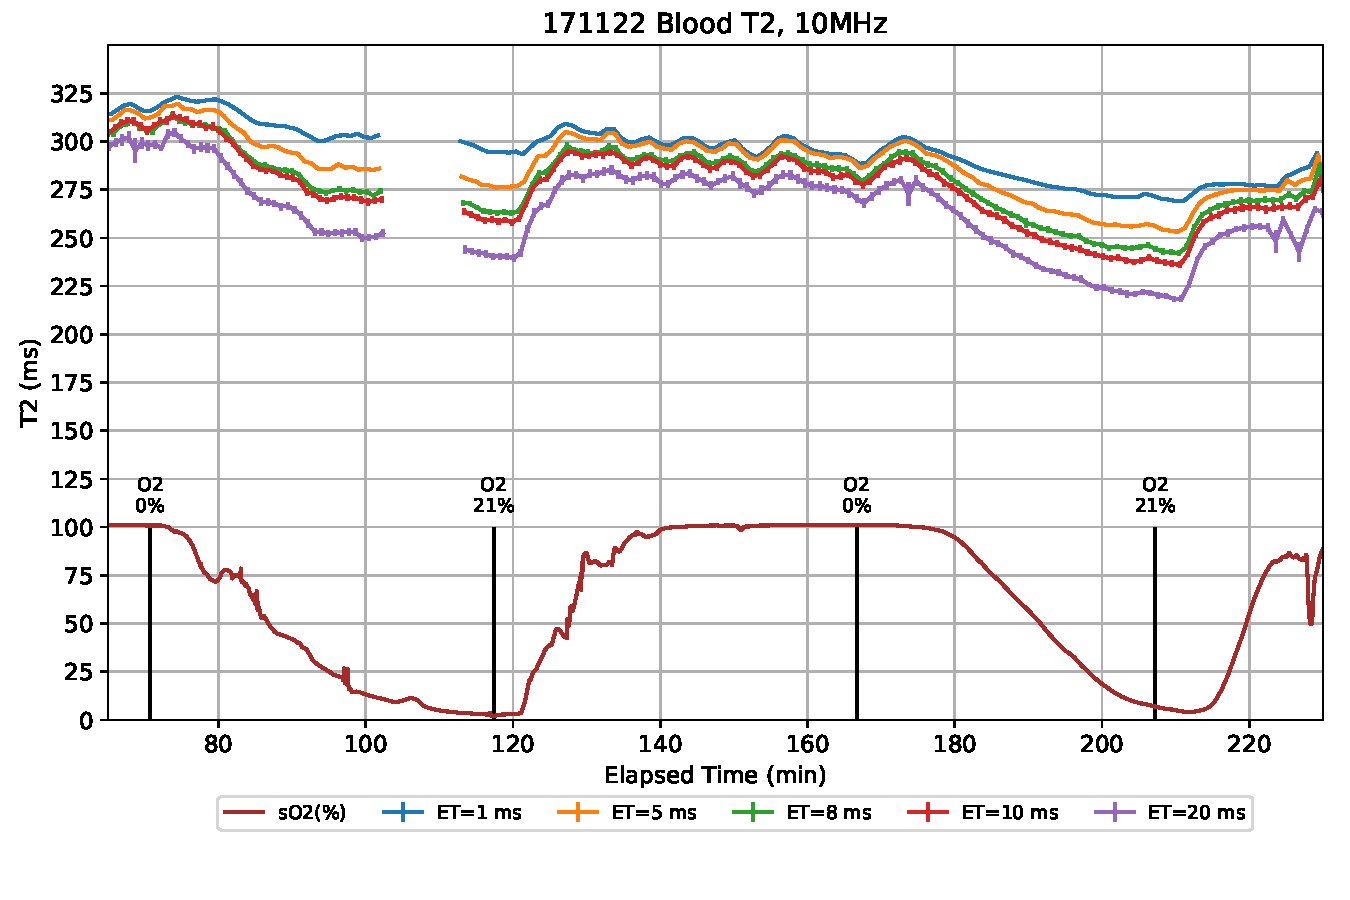
\includegraphics[width=1.2\textwidth]{figures/contflow/10MHzT2Time.pdf}}
\caption[\Ttwo measurements during blood oxygenation ramping at 10 MHz field]{\Ttwo measurements during blood oxygenation ramping at 10 MHz field. Error bars show \Ttwo fitting error. Hct =TODO - check iStat. v=\SI{1.6 \pm 0.1}{cm/s} between  70-230 minutes. Temperature was stable at \SI{28 \pm 0.5}{\celsius} during experiment.}
\label{fig:contflow-10mhzT2Time}
\end{figure}

The blood sample used in the 10 MHz experiment was collected 13 days beforehand.
The results are shown in \autoref{fig:contflow-10mhzT2Time}.

The initial \Ttwo in this experiment is around \SI{3250}{ms}.
At this oxygenation stage, there is a \SI{20}{ms} split in the \Ttwo between short and long echo times.
In other experiments, this splitting was negligible, so this effect may be due to a change in the experimental setup at this field e.g. the magnet shimming, or a higher flow rate setting.

As the \SOtwo is decreased, the \Ttwo falls from \SI{325}{ms} to \SI{300}{ms} at the \SI{1}{ms} echo time, and from \SI{300}{ms} to \SI{250}{ms} at the \SI{20}{ms} echo time.
The split increases to approximately \SI{50}{ms} when deoxygenated, which is smaller than the \SI{80}{ms} found at 14 MHz.
In the second oxygenated stage, the \Ttwo at the \SI{1}{ms} echo time is slightly lower than the initial value.
Additonally, the same splitting occurs between the short and long echo times as the first oxygenated stage.

Interestingly, this shows oscillations in the \Ttwo value between minute 120-160 .
These are well correlated with an oscillation in the blood temperature, which varied between \SIrange{27}{28}{\celsius}.
This oscillation was not observed in the other samples, and the size of the temperature dependence is larger than would be expected from other experiements (see 5 MHz data).

In the second deoxygenated stage, the \Ttwo values are \SI{20}{ms} lower than the first deoxygenated stage.
The splitting between short and long echo times remains \SI{50}{ms}.
After reoxygenation, the third oxygenated stage is lower again by \SI{23}{ms}.
These are the same sort of decreases observed in the higher field experiments.

Both deoxygenation ramps produced the expected smooth decrease in \Ttwo, so both were used for further analysis.


\subsection{5 MHz}
%Generated in processbloodoxygenation2/171129 5mhz
\begin{figure}[h!t]
\centering
\makebox[\textwidth][c]{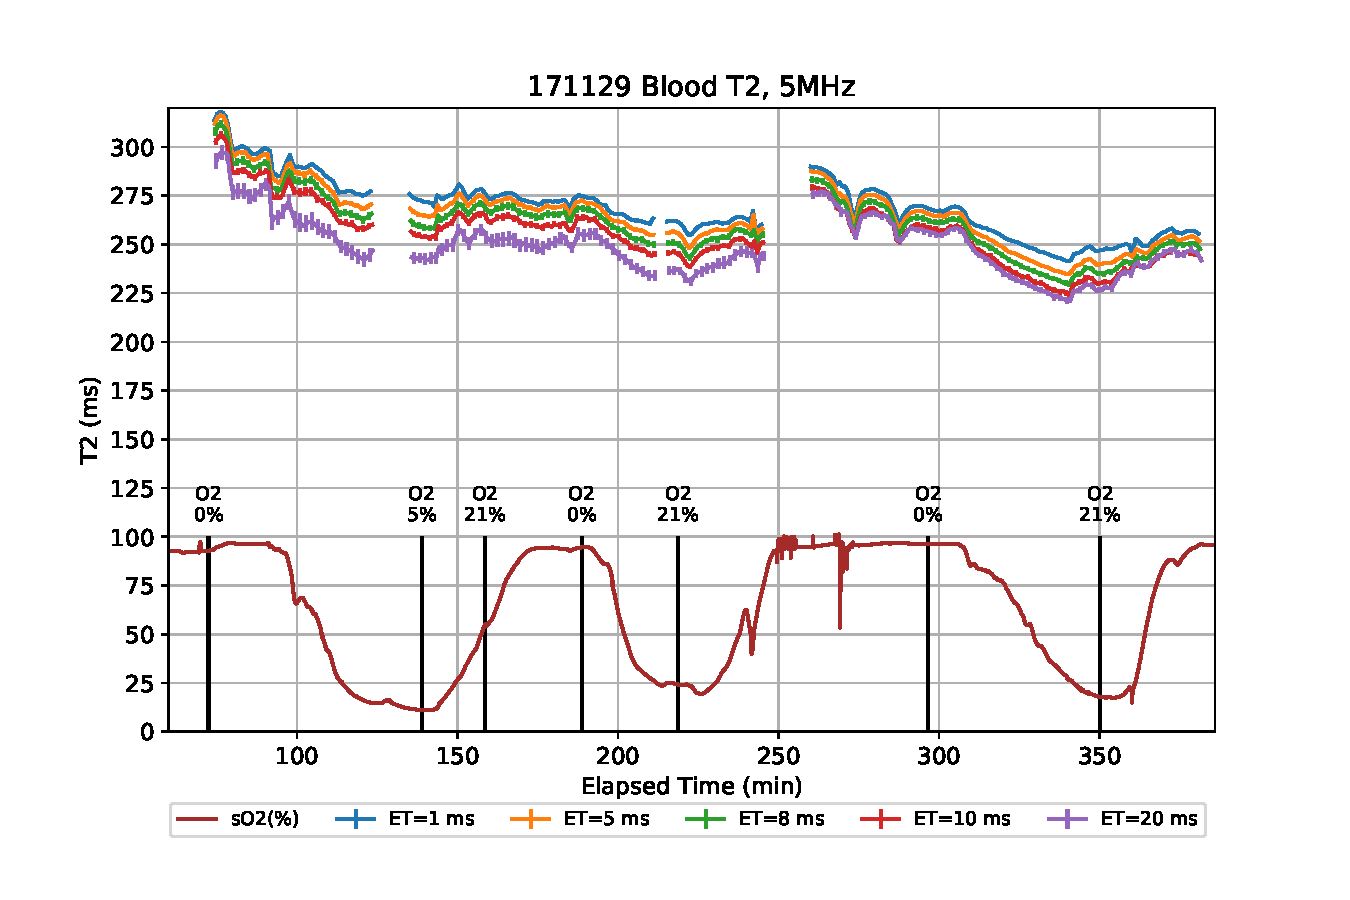
\includegraphics[width=1.2\textwidth]{figures/contflow/5MHzT2Time.pdf}}
\caption[\Ttwo measurements during blood oxygenation ramping at 5 MHz field]{\Ttwo measurements during blood oxygenation ramping at 5 MHz field. Error bars show \Ttwo fitting error. Hct =TODO - check iStat. v=\SI{2.3 \pm 0.4}{cm/s} between 80-250 minutes, and varied from \SI{1.4 \pm 0.3}{cm/s} between 280-380 minutes. Temperature varied around \SI{29 \pm 3}{\celsius} during experiment, with a drop to \SI{25}{\celsius} at 273 minutes.}
\label{fig:contflow-5mhzT2Time}
\end{figure}

The blood sample used in the 5 MHz experiment was collected the day before.
Results at the 5 MHz field are shown in \autoref{fig:contflow-5mhzT2Time}.

The initial \Ttwo for this sample is at \SI{286}{ms} for the \SI{1}{ms} echo time.
Like the 10 MHz experiment, the \Ttwo values for  short and long echo times show a \SI{20}{ms} split.

When the \SOtwo is dropped, the \Ttwo also decreases from \SI{300}{ms} to \SI{286}{ms} for the \SI{1}{ms} echo time, and from \SI{266}{ms} to \SI{232}{ms} for the \SI{20}{ms} echo time.
The \SI{20}{ms} drop at short echo time is roughly the same as the stopped flow experiment, which decreaed by \SI{25}{ms} when samples were deoxygenated.

The splitting between short and long echo times is only \SI{30}{ms} which is quite close to the splitting in the first oxygenated stage (at 90 minutes).
During reoxygenation, the small size of the \Ttwo change means that it does not appear to come back up, as the background \Ttwo decrease is of the same size at this point.
However the splitting between the \SI{1}{ms} and \SI{20}{ms} echo times returns to \SI{20}{ms}.
In the second oxygenated and deoxygenated stages, the same change in splitting occurs, even though the absolute \Ttwo value is still decreasing.

After noticing the relatively high flow rate, the flow rate was lowered from around \SI{2.3}{cm/s} to \SI{1.4}{cm/s} at 265 minutes.
The \Ttwo increases to \SI{290}{ms}, which is expected as high flow rates decrease the observed \Ttwo.
Interestingly, this also caused the splitting between the short and long echo times to decrease to around \SI{10}{ms}.

Dips at minutes 273 and 286 occur at the same time the temperature dipped \SI{4}{\celsius}, due to changing the settings on the flow rate through the oxygenator.
When the blood is deoxygenated to \SOtwo = 17\%,  the \Ttwo for the \SI{1}{ms} echo time decreases from \SI{260}{ms} to \SI{245}{ms}.
The splitting between short and long echo times increases to \SI{20}{ms} at the maximum (around minute 350).
This \Ttwo change due to oxygenation is approximately the same size as the change observed at the faster flow rate.

When reoxygenated, the \Ttwo increases back to \SI{255}{ms} at the \SI{1}{ms} echo time, and \SI{245}{ms} at the \SI{20}{ms} echo time.
The splitting of \SI{10}{ms} is consistent with the value when it was oxygenated.

Because of the change in flow rate, only the data from the second deoxygenation ramp was extracted for further analysis.

\subsection{Dependence on \SOtwo}
\label{contflow:fieldcomp}
To compare the change in \Ttwo from experiments with different field strengths, data points from the smooth, monotonic parts of the \Ttwo curves were extracted and matched with the \SOtwo measurements from the optical sensor.
This matching process took into account the delay between the optical sensor and the NMR probe.
Where data was taken from multiple oxygenation ramps, the \Ttwo values were shifted up, so that \Ttwo of oxygenated blood matched the intial measurements.
This removes the effect of the background changes in \Ttwo (effectively \TtwoO in the Luz-Meiboom equation).
These results are shown in \autoref{fig:contflow-R2SO2}.

\begin{figure}[h!p]
  \makebox[\textwidth][c]{
  \begin{subfigure}[t]{0.6\textwidth}
  \caption{40 MHz: v=1.0 cm/s}
  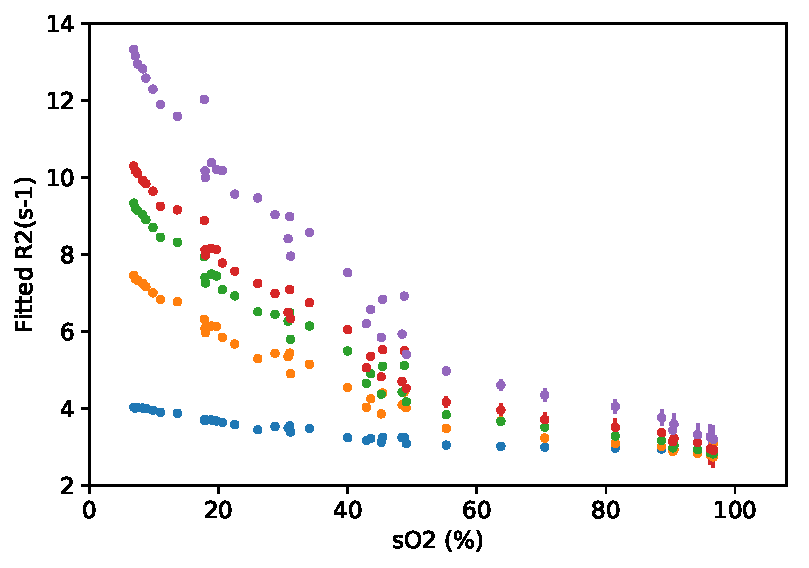
\includegraphics[width=\textwidth]{figures/contflow/40MHzR2SO2.pdf}
  \label{fig:contflow-40MHzR2SO2}
  \end{subfigure}
  \begin{subfigure}[t]{0.6\textwidth}
  \caption{20 MHz: v=1.9 cm/s}
  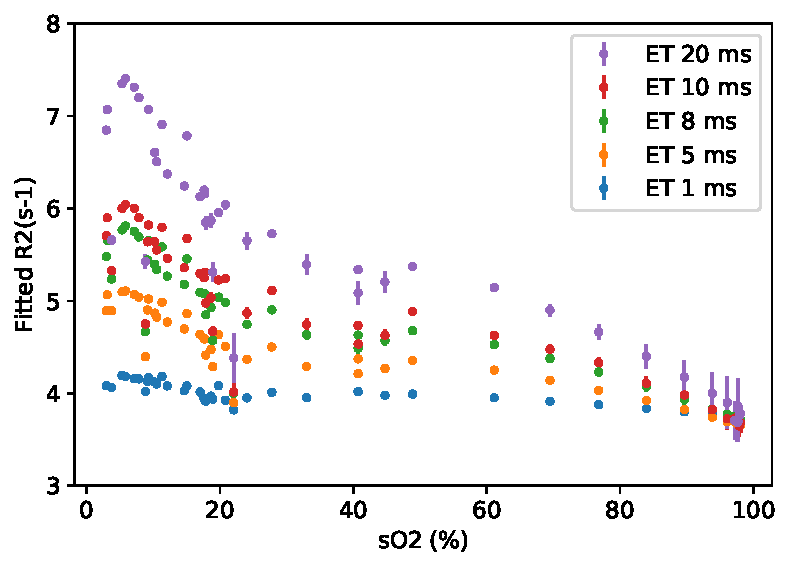
\includegraphics[width=\textwidth]{figures/contflow/20MHzR2SO2.pdf}
  \label{fig:contflow-20MHzR2SO2}
  \end{subfigure}
  \hfill
  }

  \makebox[\textwidth][c]{
  \begin{subfigure}[t]{0.6\textwidth}
  \caption{14 MHz: v=1.1 cm/s}
  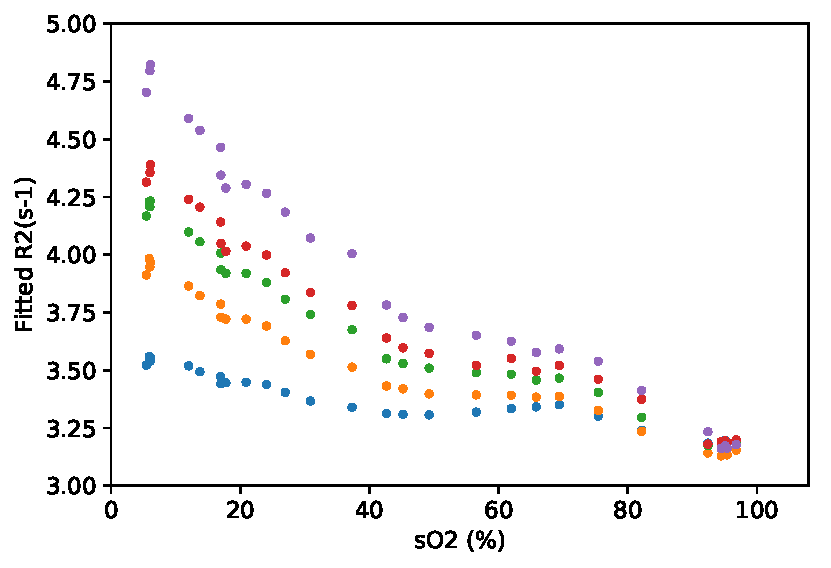
\includegraphics[width=\textwidth]{figures/contflow/14MHzR2SO2.pdf}
  \label{fig:contflow-14MHzR2SO2}
  \end{subfigure}
  \begin{subfigure}[t]{0.6\textwidth}
  \caption{10 MHz: v=1.6 cm/s}
  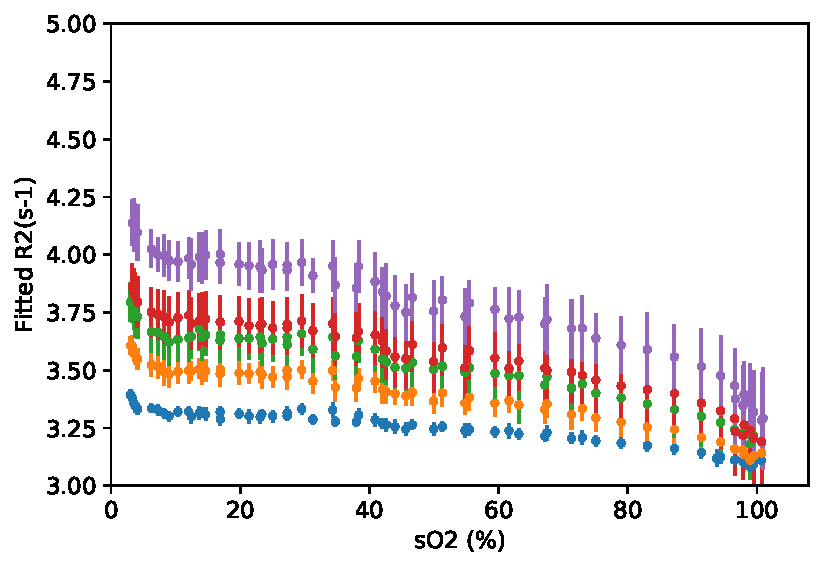
\includegraphics[width=\textwidth]{figures/contflow/10MHzR2SO2.pdf}
  \label{fig:contflow-10MHzR2SO2}
  \end{subfigure}
  \hfill
  }

  \makebox[\textwidth][c]{
  \begin{subfigure}[t]{0.6\textwidth}
  \caption{5 MHz: v=1.4 cm/s}
  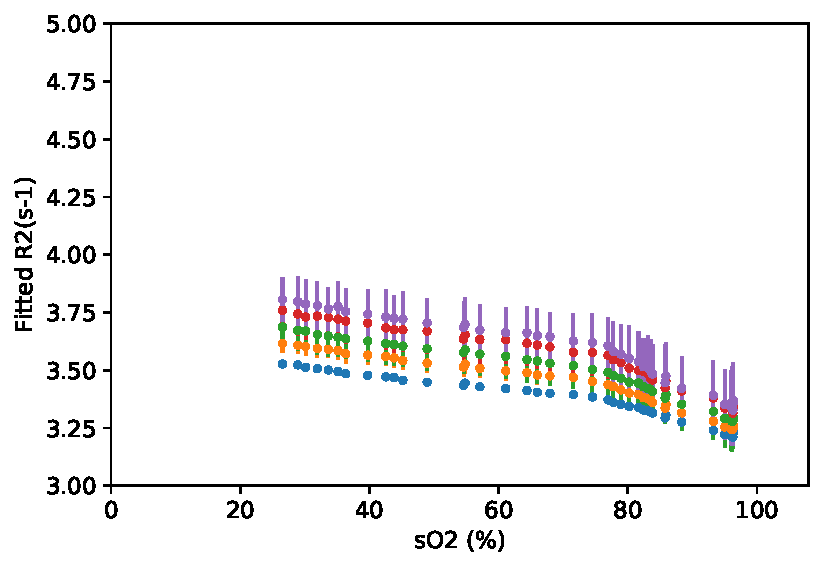
\includegraphics[width=\textwidth]{figures/contflow/5MHzR2SO2.pdf}
  \label{fig:contflow-5MHz-R2SO2}
  \end{subfigure}
  \hspace{0.6\textwidth}
  }

  \caption[\Rtwo vs \SOtwo at different field strengths]{\Rtwo during oxygenation ramps plotted against measured \SOtwo, at different field strengths. Error bars show fitting error. Note different \Rtwo scales for 40 MHz and 20 MHz data. The same symbols are used in all graph}
  \label{fig:contflow-R2SO2}
\end{figure}

These plots clearly show the increases in \Rtwo (decrease in \Ttwo) as \SOtwo decreases.
The higher field strengths also have a much wider range in \Rtwo, where the 40 MHz experiment has \Rtwo values between \SIlist{3.5;13.5}{s^{-1}}, and the 10 MHz (d) experiment has values between \SIlist{3.2;4}{s^{-1}} (the 5 MHz experiment (e) does not reach the lower levels of \SOtwo, so has a smaller range.)
The slope of the \Rtwo curves also increases at lower values of \SOtwo, which agrees with theory, which predicts a dependence on (1-\SOtwo)\textsuperscript{2}.
This effect is more visible at higher fields, and in the 10 MHz (d) and 5 MHz (e) experiments, the data appears almost linear.

\Rtwo measurements with longer echo times are also much more sensitive to the decreasing \SOtwo.
This is because there is more time for protons to experience dephasing from the field inhomogeneity as the time between the refocusing pulses increases.
These changes were not as visible in the stopped flow experiments due to the inhomogeneity of the magnets, which caused additional dephasing.

The splitting between long and short echo times also increases as \SOtwo decreases.
This also agrees with the LM model, as it predicts a higher relaxation rate at longer echo times, and .
The splitting is more visible at higher fields, as induced field inhomogeneity becomes stronger.
However, at the 5 MHz field (e), changes in \Rtwo across echo time are small enough to be within the uncertainty from fitting.

\subsection{Field Comparison}
\begin{figure}[ht]
%Graph from oxydeoxy field comparison
\centering
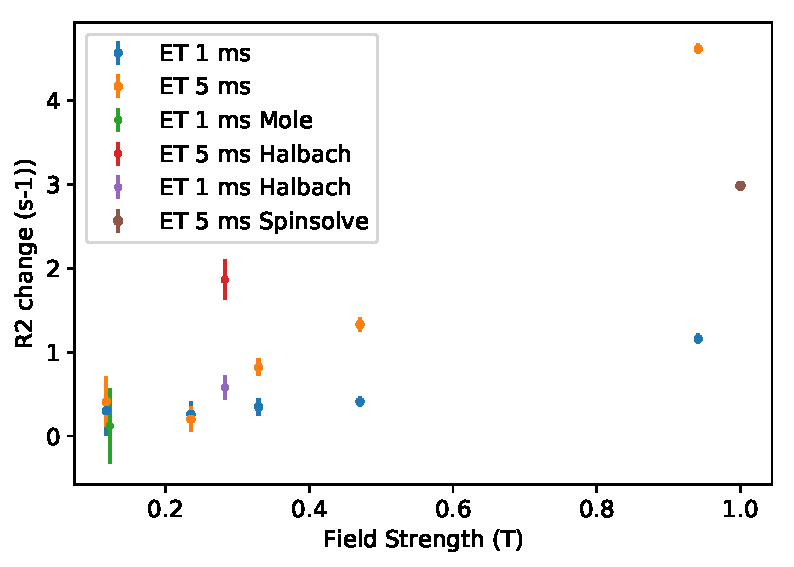
\includegraphics[width=0.8\textwidth]{figures/contflow/R2fieldDep.pdf}
\caption[Change in \Rtwo at different fields]{Change in \Rtwo at different fields for \SIlist{1;5}{ms} echo times, also showing stopped flow results at these echo times. Data points show \Rtwo\textsubscript{\textit{deoxy}} -- \Rtwo\textsubscript{\textit{oxy}}. Deoxygenated sample in 5 MHz data had \SOtwo = \SI{8}{\percent}, all others had \SOtwo < \SI{5}{\percent}}
\label{fig:contflow-R2diff}
\end{figure}

Plotting the difference in \Rtwo between deoxygenated and oxygenated blood shows the same trends.
\autoref{fig:contflow-R2diff} shows that \Rtwo change increases with field strength, going from \SI{0.35\pm0.3}{s^{-1}} at \SI{0.1}{T} to \SI{1.14\pm0.06}{s^{-1}} at \SI{1}{T} for the \SI{1}{ms} echo time.
As expected, the \SI{5}{ms} echo time shows a larger \Rtwo change, increasing to \SI{4.6\pm0.06}{s^{-1}} at \SI{1}{T}.
The trend from both echo times look quadratic enough.. TODO more scientific.

While this falls within the uncertainty of the result from the stopped flow experiment on the MOLE, the Halbach measured a slightly larger \Rtwo change at both echo times.
This may be due to effects from the background gradients not being completely removed when subtracting the relaxivities.
Conversely, the Spinsolve measurement at \SI{5}{ms} echo time is about half as large (\SI{2.96}{s^{-1}}) than the measurement at \SI{1}{T}.
The deoxygenated Spinsolve sample had \SOtwo=9\%, rather than the 4\% of the continuous flow experiment.
Taking the measured \Rtwo for this \SOtwo=9\%  from the continuous flow experiment makes the relaxivity difference \SI{4.1}{s^{-1}}, which is still larger than the Spinsolve result.

Fitting these \Rtwo measurements across different echo times to the Luz-Meiboom equation at each \SOtwo value gives a value of \Kzero for each \SOtwo.
This parameter describes the splitting between the echo times, and inspecting \autoref{eq:LMblood} and \autoref{eq:LMsimp} shows it is proportional to:
\begin{displaymath}
\gamma^2 K_0 = (Hct)(1-Hct)(1-sO_2)^2 \alpha \omega^2
\end{displaymath}

Each data point in the \Rtwo vs \SOtwo curves was fitted using non-linear fitting to find \Kzero, using  \Texc =  \SI{3}{ms} for the exchange time, and \TtwoO as a second fitted variable.
Fitting the Luz-Meiboom equation to the different \Rtwo values at the 5 echo times gave good agreement to the data across all \SOtwo values.
These results are included in \autoref{fig:contflow-K0field}.
\begin{figure}[t]
%Graph from oxydeoxy field comparison
\centering
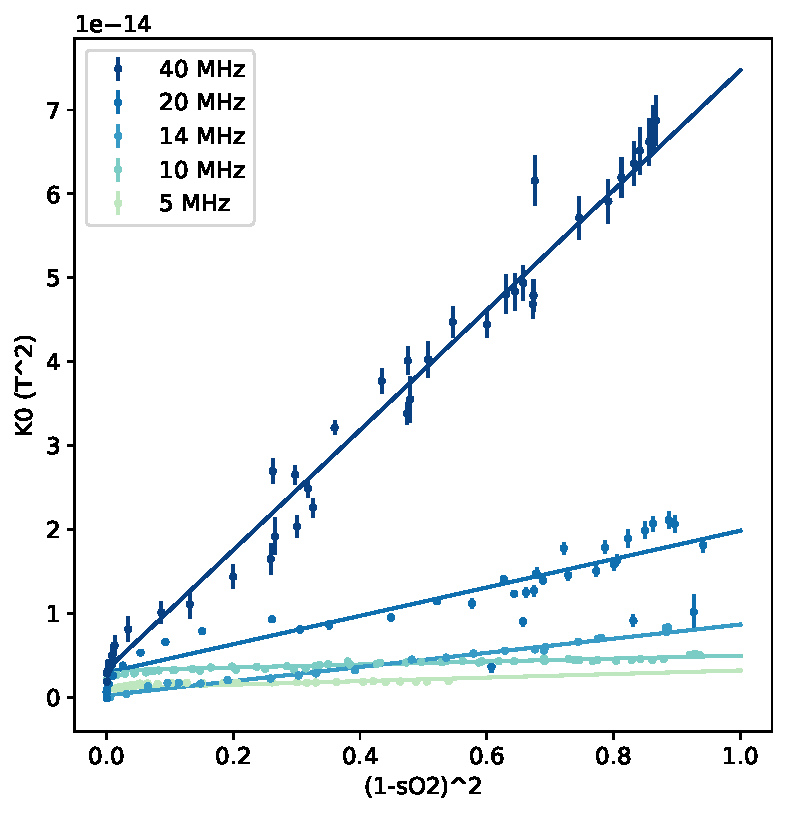
\includegraphics[width=0.8\textwidth]{figures/contflow/K0field.pdf}
\caption[Relationship between \Kzero on \SOtwo at different fields]{Dependence of \Kzero on \SOtwo at different fields. \Kzero values found by fitting as described in text. Linear fit coefficients are included in \autoref{tab:contflow-K0fitPar}. Note 5 MHz data only extends to \SOtwo=25\%.}
\label{fig:contflow-K0field}
\end{figure}

\begin{table}[b]
%data from oxydeoxy field comparison

\centering
\begin{tabular}{|c|cc|c|}
\hline
 Field (\si{MHz}) & Slope (\SI{e-14}{T^2}) & Intercept (\SI{e-14}{T^2}) & \textit{r\textsuperscript{2}} \\ \hline
5 & \num{0.21\pm0.02} & \num{0.11\pm0.00} & 0.91 \\ 
10 & \num{0.18\pm0.01} & \num{0.32\pm0.00} & 0.60 \\ 
14 & \num{0.84\pm0.03} & \num{0.02\pm0.01} & 0.95 \\ 
20 & \num{1.69\pm0.13} & \num{0.30\pm0.05} & 0.79 \\ 
40 & \num{7.15\pm0.18} & \num{0.33\pm0.07} & 0.94 \\ 
\hline
\hline
\end{tabular}
\caption[Fit parameters for dependence of \Kzero on \SOtwo]{Fit parameters showing dependence of \Kzero on \SOtwo. Plotted in \autoref{fig:contflow-K0field}}
\label{tab:contflow-K0fitPar}
\end{table}

Plotting \Kzero against (1-\SOtwo)\textsuperscript{2} shows a linear relationship at all field strengths, as predicted by theory.
These were fit using weighted least-squares fitting to find the slope.
Fit parameters for the linear fits are shown in \autoref{tab:contflow-K0fitPar}.
At high values of \SOtwo (left side of graph), the fitted \Kzero parameters should decrease to 0, as the dependence on echo time and therefore the splitting between \Ttwo values should go to zero.
In cases where oxygenated blood samples created splitting, for example the 10 MHz data, this is reflected in the intercept parameter being non-zero.

As expected, the slope also increases with field strength.
To determine the dependence on \Bzero, the slopes can be plotted on a log-log scale to see if they follow a linear trend.
This is shown in \autoref{fig:contflow-k0loglog}.
The line of best fit gives the equation log(\textit{m}) = \num{2.1\pm0.4} log(\Bzero) - \num{30.1\pm0.4}.
This is consistent with a dependence on \Bzero\textsuperscript{2}.

\begin{figure}[tbh]
%Graph from oxydeoxy field comparison
\centering
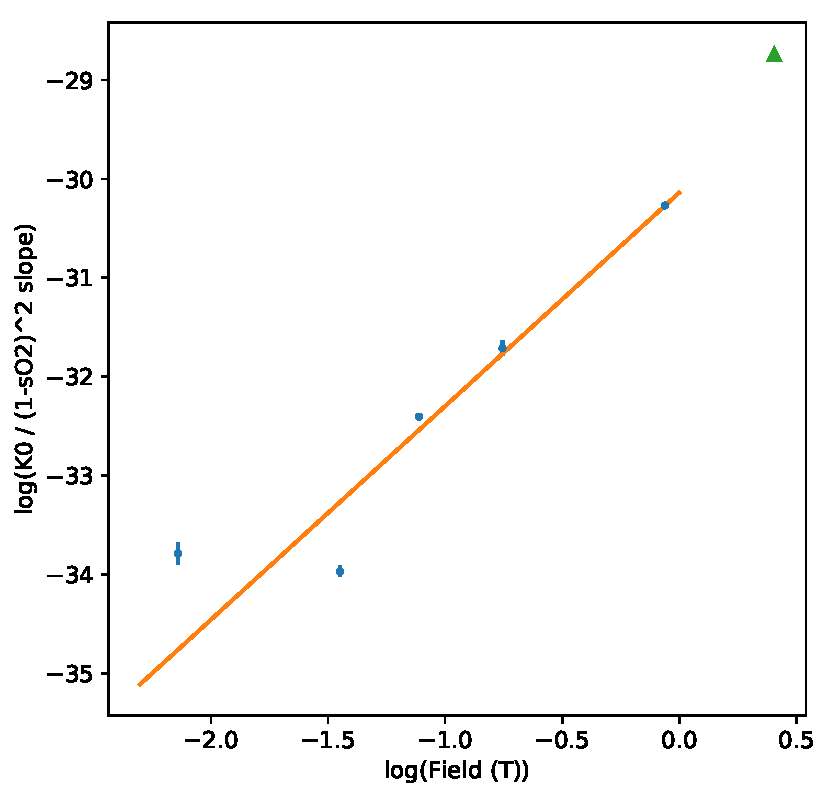
\includegraphics[width=0.6\textwidth]{figures/contflow/k0slopefield.pdf}
\caption[\Kzero slope dependence on \Bzero]{Log-log plot of \Kzero slope against field strength. Green point is included from Stefanovic et al. for comparison \cite{StefanovicHumanwholebloodrelaxometry2004}}
\label{fig:contflow-k0loglog}
\end{figure}

\section{Discussion}
%Comparison with theory
These continuous flow experiments show that decreases in blood \SOtwo cause decreases in \Ttwo, and that these changes are still visible at lower field strengths.
The \Ttwo decrease is larger when measured with longer echo times, and at higher fields, which agrees with theory.

The Luz-Meiboom equation \autoref{eq:LMblood} describes the change in \Ttwo as a function of \SOtwo, \Bzero ($\omega_0$), CPMG echo time, and haematocrit (not tested in these experiments).
In particular, it predicts that $R_2 \propto \left[\omega_0\alpha(1-sO_2)\right]^2$.
\autoref{fig:contflow-R2SO2} shows the dependence of \Rtwo in \SOtwo, which at the higher fields (40-14 MHz) appears to follow the dependence on $(1-sO_2)^2$.
Removing the effect of echo time, by fitting \Kzero to the different experiments, makes it easier to see this dependence in \autoref{fig:contflow-K0field}.
The fit results show that there is a significant linear correlation in the the parameters at most of the different field strengths.

Additionally, fitting a log-log plot of the slopes of \Kzero against the field strength \Bzero gives a slope of \num{2.1\pm0.4}.
This agrees with the theoretical dependence on \Bzero squared.
The relationship seems to hold for all but the lowest field strength (5 MHz), where the slope does not change significantly when compared to the 10 MHz slope.
This suggests that the splitting  in \Ttwo due to \SOtwo at the 5 MHz field may be too small to be picked up with this set of 5 echo times.
The dependence of echo time on \Ttwo has been investigated in more detail in \autoref{ch:models}, using a larger number of echo times.

\subsection{Confounding factors}

Other factors may also influence the \Ttwo measured in these experiments, and may add more uncertainty to the results.
This includes physical parameters such as temperature and velocity.
The temperature of the blood in the circuit was controlled using flow from \SI{37}{\celsius} water bath through the oxygenator, although because of variations in the blood flow rate through the oxygenator, the mixing process which occured in the blood bags, and changes in the room temperature, in most cases the temperature was only stable within a 3-\SI{4}{\celsius} range.
In some experiments, a stable steady-state temperature was reached, which is the ideal case.

There are a number of examples in the experimental data where features in the temperature data are correlated with changes in \Ttwo, for example in the 5 MHz experiment (\autoref{fig:contflow-5mhzT2Time}), where a \SI{4}{\celsius} drop causes a \SI{15}{ms} dip in the \Ttwo at minute 273.
This temperature drop also causes a drop in the velocity measured by PGSE, from \SI{1.6}{cm/s} to \SI{1.0}{cm/s} (although it quickly recovers when the temperature returns to \SI{29}{\celsius}).
Interestingly the value of \Ttwo changed due to the temperature, the splitting between the \SIlist{1;20}{ms} echo times stays at \SI{130}{ms} through the dip.
From this observation, there may be  up to a \SI{15}{ms} in \Ttwo measurements across some of the experiments.

Flow velocity can also affect the \Ttwo measurements.
The experiments with doped water showed that the effect should be limited to \SIrange{10}{15}{ms} at the flow rates used.
This is typically smaller than the changes due to \SOtwo.
However, over the hours-long time frame of the experiments, the flow rate typically dropped, even without adjusting the screw clamp.
This may be due to problems with the setup, such as thermal expansion of the clamp or tubing, or the narrow gap in the tube being plugged by clotted blood.
It may also be due to changes in the blood which cause it to flow slower, such as a changing viscosity.
Interestingly, a decreasing velocity would mean that the \Ttwo should increase over time however, which is opposite to the decreasing trend visible in the data.

Flow may also cause increased dispersion, which creates different \Ttwo changes at different echo times.
This effect may have been observed in the doped water experiments, where the \SI{20}{ms} echo time \Ttwo measurements experienced a slightly larger dependence on the flow rate.
This would affect the measurements based on \Kzero, which relies on the splitting between different echo times.
While this was not taken into account in the fitting model, the \Kzero fitting showed good agreement with the measured \Rtwo values to within \SI{0.3}{s^{-1}} at the high field measurements, and within \SI{0.05}{s^{-1}} in the 14, 10 and 5 MHz experiments.

Other confounding factors include haematocrit which is in the too hard basket TODO more scientific), and variations between samples of blood.

\subsection{Comparison with literature}
\label{sec:contflow-litcomp}
As mentioned in the introduction, while there have been a number of studies of \Ttwo dependence on \SOtwo in the literature, most have been done at fields \SI{>1.5}{T}, and look at either field dependence with deoxygenated and oxygenated blood, or use one field to investigate the dependence on \SOtwo.
This makes it difficult to compare these results with what has already been done.

One comparable study was done by Brooks et al., who measured the dependence of \Ttwo on field strength between \SIlist{0.02;1.5}{T} for samples of oxygenated and deoxygenated blood\cite{BrooksComparisont2relaxation1995}.
They used a fixed echo time of \SI{4}{ms}, which should be relatively close to the \SI{5}{ms} echo time series used in this experiment.
Their samples were much smaller (\SI{0.5}{ml}) and were deoxygenated using sodium dithionite (which should completely remove Oxygen).
Brooks et al. found that the difference between deoxygenated and oxygenated blood is given by $R_2 = a + bB_0^2$, where \textit{a}=\SI{4}{s^{-1}} and \textit{b}=\SI{7.2}{s^{-1}/T}.
Thiey suggested that there is still a significant difference between the deoxygenated and oxygenated blood at low field.

In contrast the continuous flow results show a similar trend, but with a=\SI{0.11\pm0.12}{s^{-1}} and b=\SI{5.1\pm0.3}{s^{-1}/T}.
While the \textit{b} value is approximately the same, the value for \textit{a} from these results means that there is little to no change in \Rtwo at low fields.

The reason for this difference is unclear, but may be due to differences in their sample preparation.
They deoxygenated the blood chemically, which can completely remove Oxygen in the samples and drop the \SOtwo to zero.
They also state that the deoxygenated blood samples were deoxygenated and used without further processing, but the oxygenated blood samples were centrifuged, washed in saline, and resuspended in thawed plasma.

Little to no change for weak \Bzero fields was also found by Gomori et al., who found a \SI{10}{ms} \Ttwo difference between oxygenated and deoxygenated blood at \SI{0.19}{T} \cite{GomoriNMRRelaxationTimes1987} -
at a \SI{2}{ms} echo time, the oxygenated and deoxygenated blood had \Ttwo values of \SI{235\pm40}{ms} and \SI{224\pm25}{ms} (estimated from graph).
This corresponds to an \Rtwo change of \SI{0.2\pm1.1}{s^{-1}}, which agrees with the little to no change in \Rtwo at low field.

The other component of this experiment that can be compared is the dependence on \SOtwo.
Stefanovic et al. measured the \Ttwo of blood at various levels of oxygenation with a range of CPMG echo times in a \SI{1.5}{T} MRI scanner\cite{StefanovicHumanwholebloodrelaxometry2004}.
They performed the same \Kzero fitting process to calibrate \Kzero values against \SOtwo, and plotted them against the same (1-\SOtwo)\textsuperscript{2}
Their results also produced a linear dependence, with a slope of \SI{3.1\pm0.2 e-13}{T^2}.
For comparison, this data point is also included in \autoref{fig:contflow-k0loglog}, and appears to follow the field dependence trend predicted by theory.

This is nice. (TODO more scientific!)

Other studies give empirical calibration constants for the shape of the \Rtwo/\SOtwo curve (curvature in \autoref{fig:contflow-R2SO2}).
The results from these studies are used to calibrate \Ttwo measurements to \SOtwo in imaging studies using the simplified equation below.

\begin{equation}
\frac{1}{T_2} = \frac{1}{T_{20}} + K\left(\tau_{180},\omega_0\right)\left(1 - \frac{sO_2}{100}\right)
\label{eq:quadmodel}
\end{equation}

This curvature constant will be dependent on parameters such as field strength, echo time and haematocrit.
One example is from Wright, who found \textit{K}=\SI{13.4}{s^-1} at a field of \SI{1.5}{T}, and a \SI{6}{ms} echo time\cite{WrightEstimatingoxygensaturation1991}.
This value was also found by Portnoy, who also found \textit{K}=\SI{13.4}{s^-1} in blood\cite{PortnoyRelaxationpropertieshuman2017}.

%TODO Found another one! 10.1002/mrm.26835
Fitting a quadratic curve to the 40 MHz experiment gives a value of \textit{K}=\SI{5.1}{s^{-1}} at the \SI{5}{ms} echo time (the closest to the echo time used by Wright).
Extrapolating this to a \SI{1.5}{T} field by multiplying by $(\frac{\SI{1.5}{T}}{\SI{0.94}{T}})^2$ gives a value of \SI{13}{s^{-1}}, which is quite close to the published value.
This would be expected to be smaller due to the lower haematocrit, and shorter echo time.


\subsection{Background \Ttwo decrease: Haemolysis?}

The general decreasing trend in \Ttwo over the time of the experiments is still significant in these experiments.
A similar effect was also observed in the stopped flow experiments, where \Ttwo values did not fully recover after the blood samples were reoxygenated.
In these continuous flow experiments, this effect is more visible due to the longer time frames and continuous monitoring.

The stopped flow experiments suggested that the change in \Ttwo might be due to the breakdown of red blood cells in the blood.
To test this more quantitatively, the haemoglobin concentration was measured for samples of plasma, separated from blood removed from the flow circuit.
This `Plasma free haemoglobin' is an indicator for haemolysis, the breakdown of red blood cells, as the cells release their haemoglobin into the surrounding plasma. \cite{MalinauskasPlasmaHemoglobinMeasurement1997}.
Additionally, the \Ttwo for the separated plasma was measured on the Spinsolve, to see if there was any correlation with the changing \Ttwo values from the continuous flow experiment.
In studies at high fields, haemoglobin has been shown in the literature to act as a paramagnetic contrast agent \cite{GrgacTransversewaterrelaxation2017}

Plasma free haemoglobin was measured using the Kahn method, which is described in a review of haemolysis testing methods by Fairbanks\cite{FairbanksMethodsmeasuringplasma1992}.
This uses UV/Vis spectroscopy of the haemoglobin absorption peak at \SI{578}{nm} to measure the concentration.
The Harboe method was also tested: this method measures the haemoglobin absorption peak at \SI{415}{nm}, but this method requires dilution of the plasma sample.
Instead, the coefficients were multiplied to remove the assumed dilution, although this did not take into account the changes that occur in absorbance due to the precipitation/dissolution of proteins and lipids in the plasma.
Absorption spectra were measured in plastic cuvettes with a \SI{1}{cm} pathlength, using a Shimadzu UV-2600 UV/Vis spectrometer (Shimadzu, Kyoto Japan).

\begin{equation}
\mathrm{Kahn: } c_{Hb} (\si{g/L}) = 1.55A_{578} - 0.861A_{562} - 0.689A_{598}
\label{eq:Kahn}
\end{equation}
\begin{equation}
\mathrm{Harboe: } c_{Hb} (\si{g/L}) = 0.836 \times \left( 2A_{415} - A_{380} - A_{450}\right) \times \frac{1}{11}
\label{eq:Harboe}
\end{equation}

These studies were done for the 40 MHz, 10 MHz and the 5 MHz experiment.
UV/Vis spectra from the 5 MHz experiment are shown in \autoref{fig:contflow-haemolyseAbsSpect}.
As the experiment time increases, the peaks at \SI{415}{nm} and \SI{570}{nm} grow, indicating an higher haemoglobin concentration.
The \SI{415}{nm} peak also appears to flatten out and decreases in height at longer times, this may be due to other interfering substances in the plasma samples.
From these spectra, the plasma free haemoglobin at each point was calculated using equations \ref{eq:Kahn} and \ref{eq:Harboe}, and these are shown in \autoref{fig:contflow-haemolyseResult}.

\begin{figure}[t]
\centering
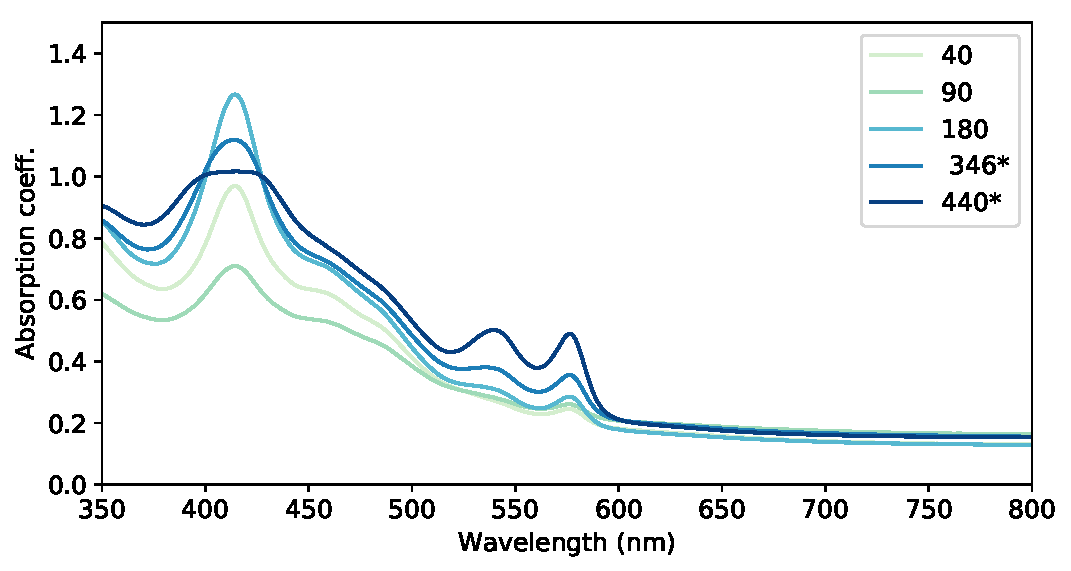
\includegraphics[width=0.9\textwidth]{figures/contflow/haemolyseAbsSpect.pdf}
\caption[Absorption spectra for samples of separated plasma in 5 MHz experiment]{Absorption spectra for samples of separated plasma in 5 MHz experiment. Different spectra sampled from circuit at time indicated. * indicates sample was taken from deoxygenated blood.}
\label{fig:contflow-haemolyseAbsSpect}
\end{figure}
The results from the 5 MHz experiment show that there is a correlation between the increasing concentration of haemoglobin, and the \Rtwo of the separated plasma.
As the concentration increases from \SI{0.05}{g/L} to \SI{0.27}{g/L}, the \Ttwo values measured in plasma decrease from \SI{757}{ms} to \SI{667}{ms}.
This corresponds to an increase in \Rtwo from \SI{1.3}{s^-1} to \SI{1.5}{s^{-1}}.
As expected, there is a large difference between the \Ttwo of the separated plasma and the blood measurements, due to the removal of the red blood cells.
Comparing this with the \Rtwo measurements in blood, this \SI{0.2}{s^{-1}} change accounts for about half of the relaxivity change between minute 90 and minute 350, which is \SI{0.4}{s^{-1}}.
\begin{figure}[h!tp]
\centering
\begin{subfigure}{\textwidth}
\caption{5 MHz experiment. (\Ttwo for blood sample at minute 350 taken from minute 294 to compare data from oxygenated blood)}
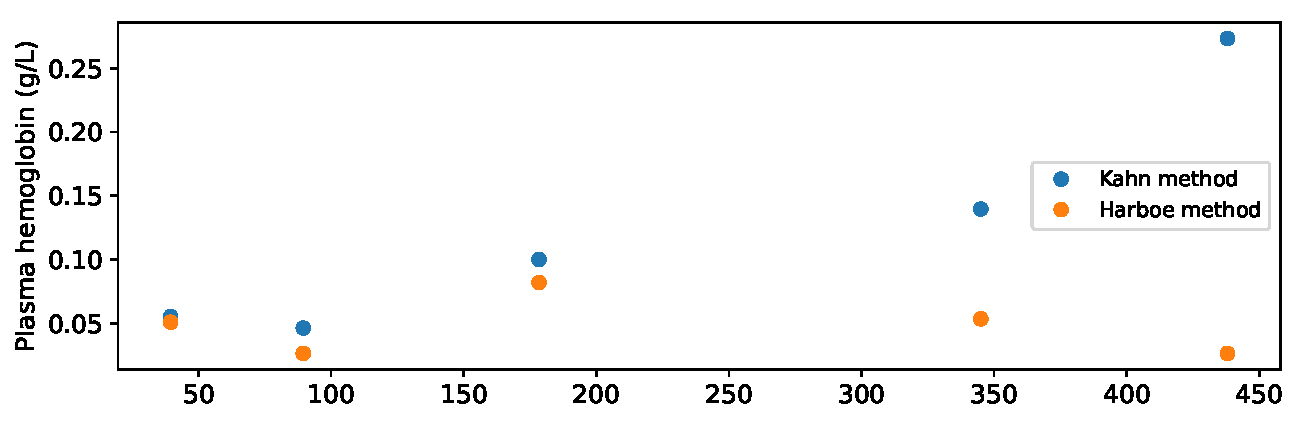
\includegraphics[width=0.9\textwidth]{figures/contflow/haemolyseSpect.pdf}

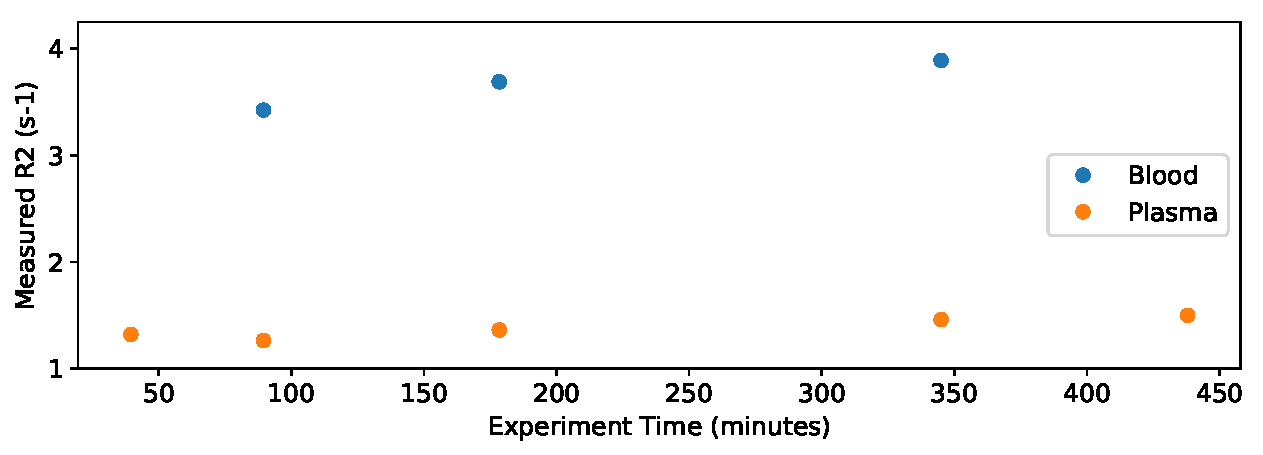
\includegraphics[width=0.9\textwidth]{figures/contflow/haemolysePlasT2.pdf}
%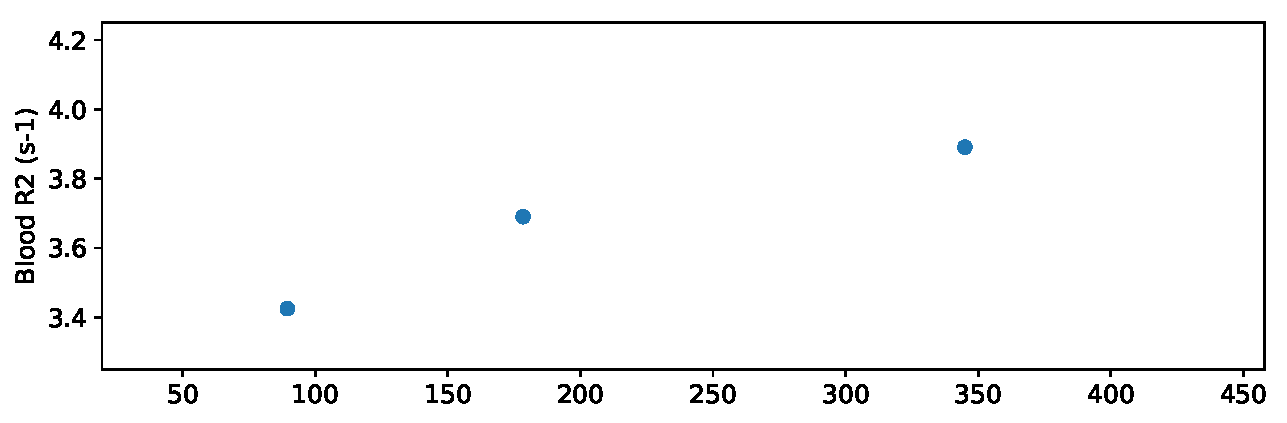
\includegraphics[width=0.9\textwidth]{figures/contflow/haemolyseBloodT2.pdf}
\end{subfigure}

\begin{subfigure}{\textwidth}
\caption{40 MHz experiment}
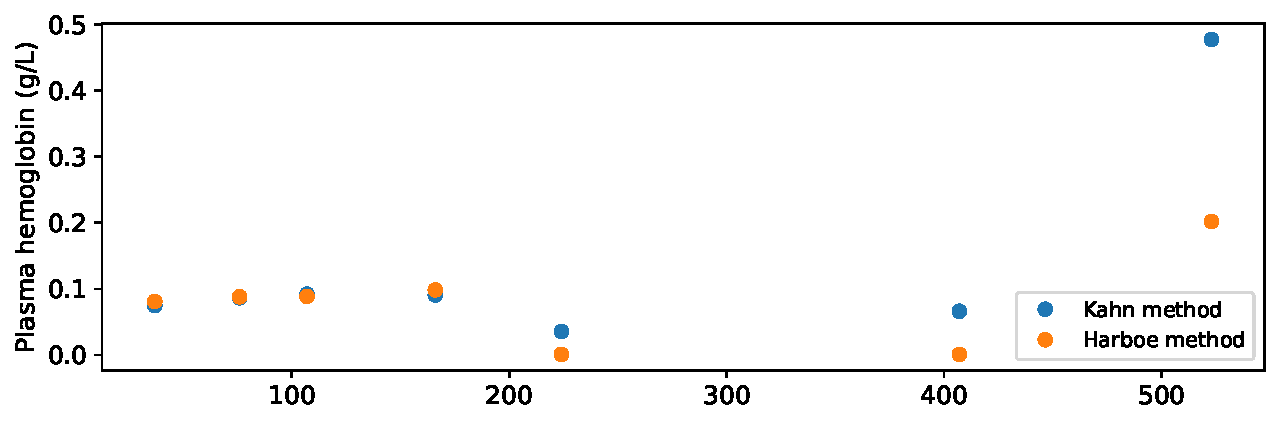
\includegraphics[width=0.9\textwidth]{figures/contflow/40haemolyseSpect.pdf}

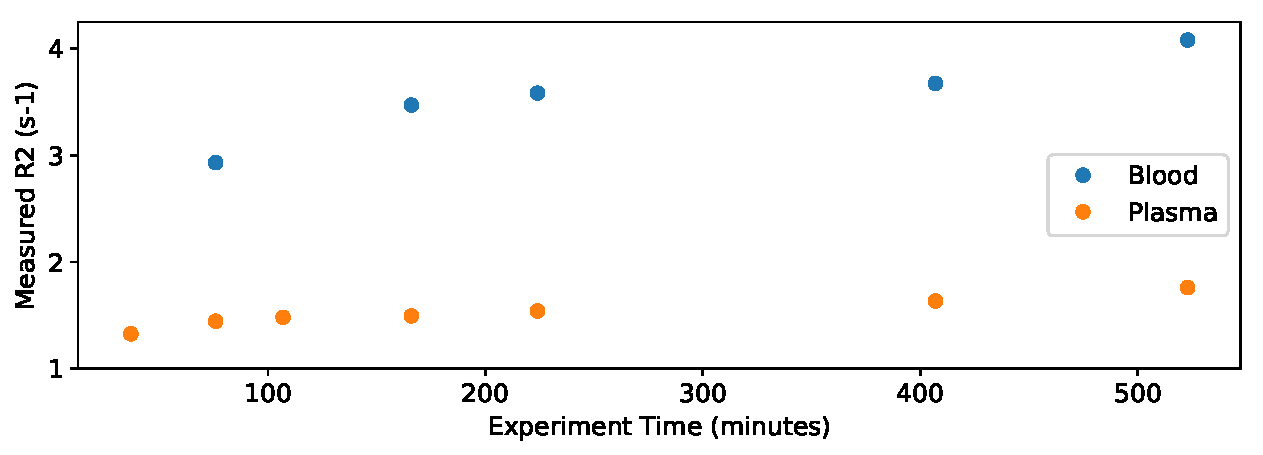
\includegraphics[width=0.9\textwidth]{figures/contflow/40haemolysePlasT2.pdf}
%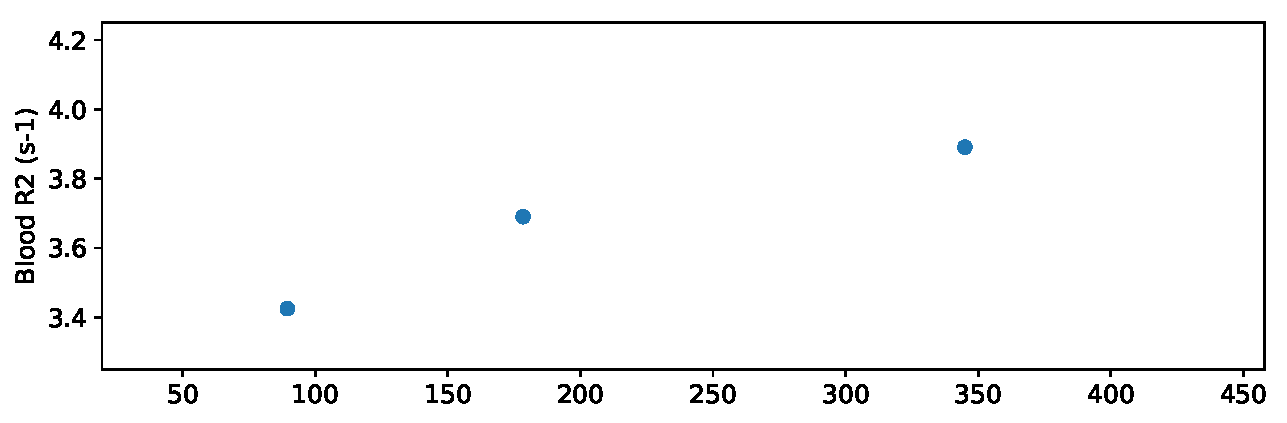
\includegraphics[width=0.9\textwidth]{figures/contflow/haemolyseBloodT2.pdf}
\end{subfigure}
\caption[Blood haemolysis experiment result]{Blood haemolysis experiment result. Plasma free haemoglobin found using Kahn method, Plasma \Rtwo values measured on Spinsolve at \SI{1}{T}, Blood \Rtwo values taken from blood data shown in \autoref{fig:contflow-5mhzT2Time} and \autoref{fig:contflow-40mhzT2Time}}
\label{fig:contflow-haemolyseResult}
\end{figure}
A similar result was found in the 40 MHz experiment, although the plasma sample used was relatively cloudy, potentially due to lipids or proteins in the plasma , which meant that the UV/Vis spectra displayed broad absorptions.
This broke (TODO more scientific!) the Kahn method, as it uses the region around the absorption peak to attempt to remove background absorption.

\Rtwo values in the separated plasma increased from \SI{1.25}{s^{-1}} to \SI{1.7}{s^{-1}}, while the oxygenated blood increased from \SI{2.9}{s^{-1}} to \SI{4.0}{s^{-1}}.
The
While the UV/Vis spectra from this experiment cannot conclusively link free haemoglobin and the plasma \Rtwo, the increasing trend in the plasma \Rtwo and blood \Rtwo over time suggest that the blood is breaking down.

These experiments suggest that the background decrease in \Ttwo across the time span of the experiments is due to haemolysis of the red blood cells.
Haemolysis can be caused by many factors including the age of the blood, changes in osmolarity, temperatures above \SI{40}{\celsius} and mechanical/shear stress\cite{Sowemimo-CokerRedbloodcell2002}
This was observed happening in the pump when the occlusion was set too tightly, which lead to the use of the occlusion setting process described in .
It is possible that haemolysis is occuring due to the blood flowing through the relatively tight screw clamp, or due to contact with the PVC tube and oxygenator membrane.
Blood haemolysis is also known to occur in \textit{ex-vivo} blood circulation circuits for cardiopulmonary bypass, although typically the natural scavenging process in the body is able to clear this without significant ill-effects\cite{VercaemstHemolysiscardiacsurgery2008}.

\subsection{\SOtwo measurement from \Ttwo}
As the goal of this project is to determine how well \SOtwo can be measured using NMR at low fields, the results from the continuous flow experiments were used to back-predict the \SOtwo for comparison to the optical sensor.
In the literature, most experiments use a calibration curve to directly link measured \Ttwo values with \SOtwo for one echo time.
This process was pioneered by Wright\cite{WrightEstimatingoxygensaturation1991}, and applied by Golay\cite{GolayMeasurementtissueoxygen2001}, Portnoy CITE[other paper] and many others.

More recently, a parametric method of fitting \Ttwo values measured at multiple echo times has been introduced by Varghese\cite{VargheseCMRbasedbloodoximetry2017} for use in MRI oximetry of the heart.
This relies on using non-linear least sqaures fitting to fit the full Luz-Meiboom equation (\autoref{eq:LMblood}, which includes terms for Hct, $\alpha$ and \SOtwo) to the measured \Ttwo values, and extracting \SOtwo from this.
In their study, they demonstrated that this parametric method improved \SOtwo measurement accuracy when compared to the simplified calibration curve model, by comparing the \SOtwo values calculated with each method to direct \SOtwo measurements of blood sampled from the heart (in pigs).
This method requires a separate measurement of a sample of blood to find a known \SOtwo value and the haematocrit, to be able to estimate $\alpha$ and the haematocrit factor in the Luz-Meiboom equation.
\Ttwo values were measured using 4 echo times between \SIrange{10}{25}{ms}, which were used to estimate either the \SOtwo, or 4 constrained parameters: \SOtwo, Hct, $\alpha$ and \TtwoO.

In this work, a similar parametric method was applied to find \Kzero and \TtwoO from the 5 echo times in each measurement.
This should mean that effects due to temperature, flow and haemolysis should be able to be ignored, so that the \SOtwo prediction depends only on the echo time splitting.
This \Kzero value was then converted to an \SOtwo using the values in \autoref{fig:contflow-K0field}, which describe the linear relationship between \Kzero and $(1-sO_2)^2$.
In effect, this is the same as the `Approach 3' trained method described by Varghese, where the `nuisance parameters' are found from the training data, which are the slope parameter in \autoref{tab:contflow-K0fitPar}.
The short echo times used in these experiments, particularly the \SI{1}{ms} time, should allow this method to better estimate the \TtwoO, while the wide range of echo times also provides a larger splitting, allowing for better estimation of \Kzero.

This method was applied to data from the 14 MHz experiment, shown in \autoref{fig:contflow-NMRSO2}.
The section of the experiment where the \Ttwo and optical sensor \SOtwo values were extracted for analysis (effectively training data) is shown in grey.
For comparison, a quadratic \Rtwo/\SOtwo calibration was also calvulated using the value of \textit{K} found above in \autoref{sec:contflow-litcomp} and is shown in red.

\begin{figure}[t]
%Graph from 14MHz experiment
\centering
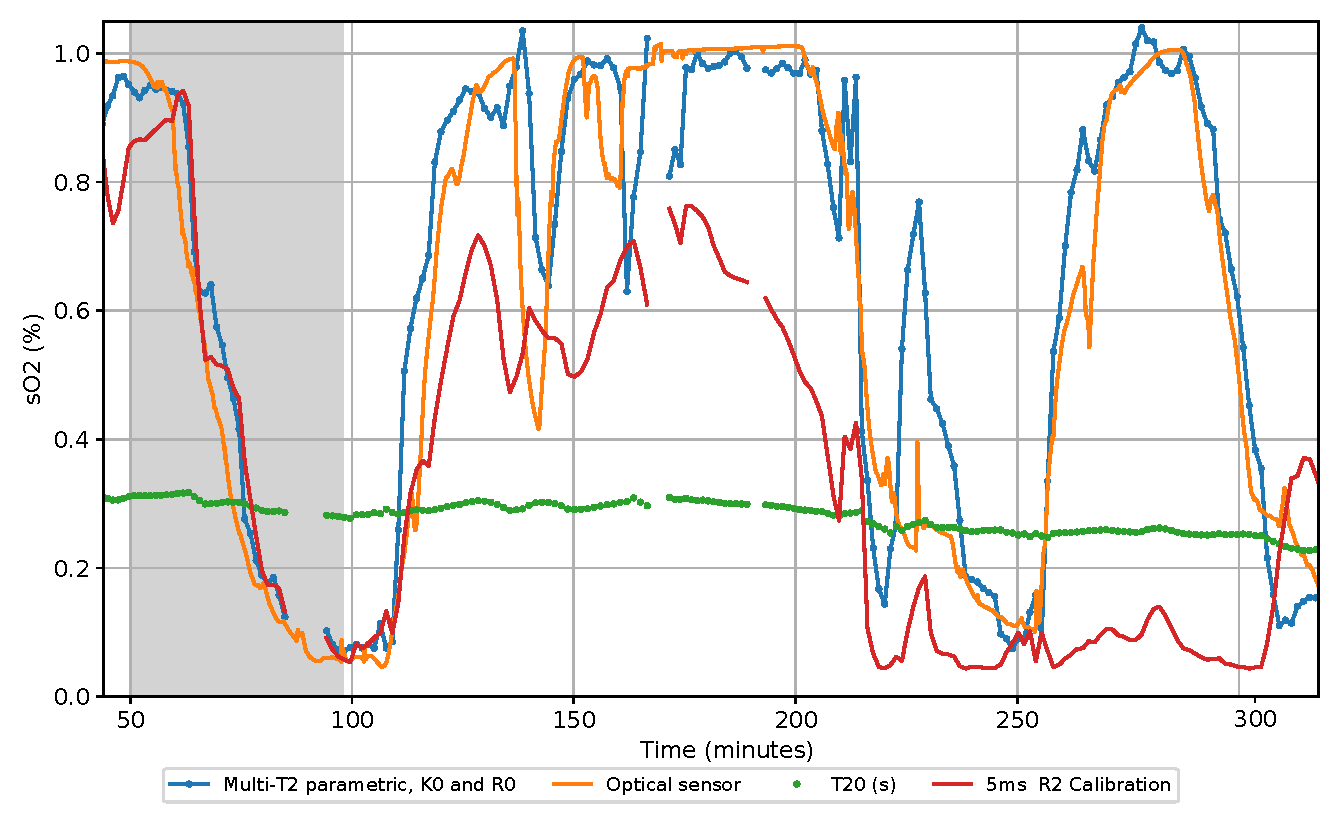
\includegraphics[width=0.8\textwidth]{figures/contflow/calibratedNMRSO2.pdf}
\caption[Back-predicted \SOtwo from NMR measurements at 14 MHz]{Back-predicted \SOtwo from NMR measurements at 14 MHz, using data highlighted in grey as `training' data}
\label{fig:contflow-NMRSO2}
\end{figure}

This demonstrates that the \SOtwo calculated by the parametric method tracks the optical sensor measurement well, and is not affected by the background changes in \Ttwo.
It also shows that the quadratic calibration curve follows the optical sensor data, but is significantly biased towards lower \SOtwo as the experiment continues, due to the background decrease in \Ttwo.
The background decrease is shown by the decreasing \TtwoO line, which decreases from \SI{305}{ms} to \SI{250}{ms}.
Interestingly, the spikes where sudden changes in oxygenation occured (e.g. minutes 140, 225) have a different shape in the NMR data to the optical sensor data.
This could indicate that there is some sort of change in the \SOtwo as the blood travels between the optical sensor and the probe.

The data also shows that the size of the splitting is not affected by the haemolysis -- increased concentrations of haemoglobin in plasma could be expected to decrease the susceptibility differences between the blood cell cytoplasm and the plasma, causing the strength of the \Ttwo shortening effect to decrease.
This would lead to a decreased \Kzero for the same \SOtwo, and therefore predict a higher \SOtwo.
This does not appear to be the case, for example at minute 250, where the optical and NMR data are still in good agreement, suggesting that the free haemoglobin is not at a high enough level to affect the field inhomogeneity.

These continuous flow experiments show that changes in \SOtwo can be detected using \Ttwo at low field, and that the trends in \Ttwo agree with the literature.
While the temperature and flow effects in the experiments may need to better controlled, the results still appear to follow the expected trends.
Repeating these experiments with more samples of blood will also be needed to confirm these results, as they come from one sample at each field strength.
Additionally, we have found evidence that blood is breaking down during the course of the experiments, suggesting that this \Ttwo method could be sensitive for this.
